\chapter{General introduction on the diseases of interest}
\label{chapter:introduction}
\chaptermark{General introduction}

%%%%%%%%%%%%%%%%%%%%%%%%%%%%%%%%%%%%%%%%%%%%%%%%%%%%%%%%%%%%%%%%%%%%%%%%
%%%%%%%%%%%%%%%%%%%%%%%%%%%%%%%%%%%%%%%%%%%%%%%%%%%%%%%%%%%%%%%%%%%%%%%%
%%%%%%%%%%%%%%%%%%%%%%%%%%%%%%%%%%%%%%%%%%%%%%%%%%%%%%%%%%%%%%%%%%%%%%%%
% overall intro on the topic
% \note{General intro on the overall topic}
The advances made in the medical field over the last century have brought significant benefits to human society. Progress, such as the eradication of diseases through the development and deployment of effective vaccines, reduction of bottleneck-like diseases, such as malaria, and the ability to manage once life-threatening diseases into chronic states (e.g., diabetes, human immunodeficiency viruses, and some forms of cancer) has significantly improved the overall life expectancy and quality of life. This progress is particularly noticeable in Western countries. However, this modern and long-lasting society has also given rise to cultural changes that are beginning to manifest. Lifestyle changes such as promoting increased protection by increasingly reducing contact with external pathogens and gradually extending working hours under more stressful conditions, coupled with continuous exposure to potential new environmental risk factors, have led to a prevalence increase in autoimmunity and complex new diseases.
% and the rise of global pandemics.

% \note{ME/CFS}
This thesis aims to enhance our understanding of Myalgic encephalomyelitis/Chronic fatigue syndrome (\cfs) as a disease with immune dysregulation, akin to other autoimmune conditions. Additionally, it discusses alternative stratification strategies based on distinct mechanisms, such as symptom severity or infection triggers. Our focus includes analysing patterns of antibody reactivity towards specific herpesviruses and examining symptom profiles by subgrouping patients based on disease onsets. Alternatively, we categorise patients' symptoms into domains and explore different hypothesised aetiologies across the sampled population. In the context of \cfs, we also explore methods to improve the consistency of case-control studies---widely used in studies on biomarkers and risk factors---by simulating scenarios under the assumption of imperfect diagnosis of \cfs patients (i.e., misdiagnosis). All analyses utilise available or published datasets.

% \note{\covid}
Part of the present thesis was produced during the latter half of the coronavirus disease 2019 (\covid) pandemic. This was an unprecedented global event with a worldwide impact, which also influenced the focus of research produced at the time. Here, we assessed the protection effectiveness and stability of vaccines, coupled with prior infections (i.e., hybrid immunity) against the Omicron BA.5 sub-variant over time, a worrying lineage in that period.

% Introduction to ME/CFS and SARS-CoV-2 
% \note{Concluding and what goes in this chapter}
Before delving into the discussion of this thesis, it is necessary to provide proper introductions to both topics of \cfs as a heterogeneous disease and the research interest of the severe acute respiratory syndrome coronavirus 2 (\sars) virus in the context of the pandemic, as well as delineating the objectives of the thesis. Initially, background information on the importance of stratifying \cfs patients to identify more consistent patient groups and implement precise and personalised treatments is provided (\textbf{Section~\ref{sec:background-mecfs}}). Then, a brief introduction to the \sars virus, \covid pandemic, and the challenges posed by rising variants of concern over time is given (\textbf{Section~\ref{sec:sars-and-covid}}). Lastly, the thesis structure and research aims are presented (\textbf{Section~\ref{sec:aims-thesis}}). This is the purpose of this general introduction.


%%%%%%%%%%%%%%%%%%%%%%%%%%%%%%%%%%%%%%%%%%%%%%%%%%%%%%%%%%%%%%%%%%%%%%%%
%%%%%%%%%%%%%%%%%%%%%%%%%%%%%%%%%%%%%%%%%%%%%%%%%%%%%%%%%%%%%%%%%%%%%%%%
%%%%%%%%%%%%%%%%%%%%%%%%%%%%%%%%%%%%%%%%%%%%%%%%%%%%%%%%%%%%%%%%%%%%%%%%
\section{Myalgic encephalomyelitis/Chronic fatigue syndrome}
\label{sec:background-mecfs}

% \note{Quick intro on the topic, no citations needed even?}
Myalgic encephalomyelitis/Chronic fatigue syndrome (\cfs) is a chronic and debilitating clinical condition with unknown aetiology and pathophysiology. The disease has a broad definition, which makes its diagnosis \red{one of exclusion}.
\red{\textbf{symptoms} + exclusion}
This allows for a large combination of symptoms with varying degrees of severity, resulting in a heterogeneous group of diagnosed patients.
Patients affected by ME/CFS report post-exertional malaise (PEM) and unexplained and persistent fatigue that is not alleviated by rest as key symptoms.
They also experience a plethora of other symptoms related to the dysfunction of immunological, autonomic, cognitive, neuroendocrine, or neurological systems.
Generally, these symptoms worsen following what would be considered normal levels of physical, mental, or emotional effort.
\red{Remove things below}
\red{Mal começo a apresentar começo logo a denegrir a doença}

\red{SNS não reconhece a doença, não os pacientes}
\red{The lack of diagnosis sensitivity}, consensual results, and overall agreement regarding the cause of \cfs has led to disinterest from both the social and medical communities that often do not view the disease as legitimate. \red{No refs no nothing}
Consequently, patients can be subjected to disregard or, at worst, even \red{disrespectful treatment} \textbf{cortar isto}.
% by the health care system
% There is also a lack of funds for its research
\red{[needs improvement? no treatment? mention lack of funding for research?]}
% \citep{anderson2014QualitativeNatural, donalek2009WhenParent, anderson1997QualityLife}


%%%%%%%%%%%%%%%%%%%%%%%%%%%%%%%%%%%%%%%%%%%%%%%%%%%%%%%%%%%%%%%%%%%%%%%%
%%%%%%%%%%%%%%%%%%%%%%%%%%%%%%%%%%%%%%%%%%%%%%%%%%%%%%%%%%%%%%%%%%%%%%%%
% \subsection{Brief history of the disease}
\subsection{Brief history of the disease}
\label{subsec:mecfs-history}

The uncertainty around \cfs as a disease extends even to its nomenclature, mirroring the long-lasting debate surrounding the definition of the disease. The terms myalgic encephalomyelitis (ME) and chronic fatigue syndrome (CFS), which nowadays collectively characterise the condition, have distinct origins.% \red{that explain the gradual understanding of this illness}.

% \note{ME}
ME generally denotes the involvement of the central nervous system and brain or spinal cord inflammation. This term was the original definition, coined in 1934 to describe multiple similar outbreaks where the afflicted individuals reported malaise, severe headaches, sore throat, myalgia, and swollen lymph nodes \citep{anderson2014QualitativeNatural}. Since then, the idea for the diagnosis has changed over time, and alternative names and definitions have emerged in continued efforts to describe the heterogeneous clinical syndrome. Examples of historic names used are chronic infectious mononucleosis \citep{isaacs1948ChronicInfectious}, Royal Free disease \citep{ramsay1956EncephalomyelitisSimulating, themedicalstaffoftheroyalfreehospital1957OutbreakEncephalomyelitis}, benign myalgic encephalomyelitis \citep{galpine1957BenignMyalgic}, epidemic neuromyasthenia \citep{henderson1959EpidemicNeuromyasthenia}, post-viral syndrome \citep{behan1985PostviralFatigue}, idiopathic chronic fatigue and myalgia syndrome \citep{byrne1988IdiopathicChronic}, and fibrositis-fibromyalgia \citep{pritchard1988FibrositisChronic, yunus1989FibromyalgiaSyndrome}.
% (names provided by \citet{sharpe1991ReportChronic} and \citet{rivera2019MyalgicEncephalomyelitis}).
% attributed in 1955 after an outbreak at the Royal Free Hospital in London that affected a large number of doctors and nurses \citep{ramsay1956EncephalomyelitisSimulating, themedicalstaffoftheroyalfreehospital1957OutbreakEncephalomyelitis}.
% A few decades later, ME was linked with psychosocial phenomenon and assumed also to have a psychiatric component.
The interpretation of ME also evolved. The term was first used to describe a post-infectious condition due to the presence of flu-like symptoms in large groups of patients. However, it was also associated with psychosocial phenomena and assumed to have a psychiatric component, linking the outbreaks with mass hysteria. It eventually became more broadly used to describe an inflammatory disease with effects on the brain, muscles, and nerves \citep{evengard2002ChronicFatigue, instituteofmedicine2015MyalgicEncephalomyelitis}.

% \note{CFS}
On the other hand, the term CFS emphasises the overwhelming fatigue experienced by patients \citep{wojcik2011ChronicFatigue}. Introduced in 1988 by the US Center for Disease Control and Prevention (CDC), CFS was intended to replace a disease termed chronic Epstein-Barr virus (EBV) syndrome\footnote{The name prior to the introduction of the term CFS reflects the link between the herpesvirus as the origin of the disease at the time, which considered a latent chronic infection as a key point for the disease. However, only a part of patients diagnosed---albeit a majority---showed high titres of IgG anti-EBV antibodies \citep{horwitz1985LongtermSerological}, making the term less inclusive.} and be a more inclusive name, free from unproven aetiological implications \citep{holmes1988ChronicFatigue}. However, this definition was eventually deemed too broad and unsatisfactory in practice since it focused predominantly on fatigue, becoming an oversimplification of the true effects and making the extensions of the disease more difficult to understand \citep{noor2021ComprehensiveUpdate}. Moreover, the term has also received complaints from patients, justifying that it ``stigmatises and trivialises'' the disease, leading to ``social disregard'' and disengagement \citep{instituteofmedicine2015MyalgicEncephalomyelitis}.
% - \textit{Post-viral (fatigue) syndrome} could be a more general name. However, similarly to Chronic EBV infection, not all diagnosed patients reported an infection as the onset for the disease, making this a not so appropriated term.
% Also, myalgia is not common to all patients, as well as encephalitis or myelitis, which is not confirmed by laboratory in most studies.

% \note{ME/CFS}
Over the past decades, distinct case definitions and diagnostic criteria have been developed for the two terms (e.g., \citet{hyde2007NightingaleMylagic, carruthers2011MyalgicEncephalomyelitis} for ME and \citet{holmes1988ChronicFatigue, sharpe1991ReportChronic, fukuda1994ChronicFatigue} for CFS) and the debate for the implementation of a unifying term remained, with additional proposals being suggested as different case definitions and diagnosis criteria were published. The more recent proposes have been neuroinflammatory and oxidative fatigue (NIOF) \citep{maes2015NewCase} and systemic exertion intolerance disease (SEID) \citep{instituteofmedicine2015MyalgicEncephalomyelitis}.

Despite the general discussion that a more appropriate name could be adopted, the composite name ME/CFS (or CFS/ME in some cases) was eventually popularised and remains the more conventional term used to describe the disease \citep{carruthers2003MyalgicEncephalomyelitis}. Thus, ME/CFS can be regarded as an umbrella term that encapsulates all conditions and adjustments considered since the initial description of the disease, even if neither ME nor CFS fully capture the complexity of the disease.
% Moreover, the usage of this term implies an underlying pathology that is yet to be validated.
% Thus, ME/CFS is an umbrella term that avoids ambiguity and includes all previously considered conditions and adjustments done since the disease was initially described.
% Since then, ME/CFS has come to serve as an umbrella term that characterised the dysregulation of systems.
% ME/CFS term \citep{jason2014ExaminingCase, carruthers2003MyalgicEncephalomyelitis}


%%%%%%%%%%%%%%%%%%%%%%%%%%%%%%%%%%%%%%%%%%%%%%%%%%%%%%%%%%%%%%%%%%%%%%%%
%%%%%%%%%%%%%%%%%%%%%%%%%%%%%%%%%%%%%%%%%%%%%%%%%%%%%%%%%%%%%%%%%%%%%%%%
% \subsection{Epidemiology of the disease}
\subsection{Epidemiology}
\label{subsec:epidemiology}
% \subsection{Disease prevalence and patient's characteristics}

% \note{Prevalence}
% ME/CFS occurs worldwide and its o
The global prevalence estimates of ME/CFS have a \red{wide amplitude, isto é um julgamento meu, não estou a reportar}.

\red{The prevalence estimates of ME/CFS is X to Y.}
Epidemiological systematic reviews and meta-analyses report values ranging between 0.1\% and 2.2\% \citep{estevez-lopez2020SystematicReviewa}, with an overall pooled estimate of 0.89\% (95\% CI = [0.60, 1.33]) \citep{lim2020SystematicReviewa}.

Só temos estudos an Europa
- Islandia
- Inglaterra
- outro

\citet{estevez-lopez2020SystematicReviewa} é um estudo europeu

% Interestingly, questionnaire-based interviews without a clinical test report even higher prevalence estimates of 1.14\% (95\% CI = [0.76; 1.72]) \citep{lim2020SystematicReviewa}.
% The application of such questionnaires can potentially overestimate the true prevalence. However, it shows an interest in participation
This variability is largely attributed to differences in the assumed disease definitions and diagnostic methods, as well as the study region \citep{vincent2012PrevalenceIncidence, nacul2011PrevalenceMyalgic, valdez2018EstimatingPrevalence, slomko2019PrevalenceCharacteristics}. Despite this uncertainty, considering the current world population of 8.1 billion humans, at least 72 million individuals worldwide are affected by this endemic disorder, present across all ethnic groups and socioeconomic strata.
% ME/CFS has been shown to affect all ethnic groups and social groups \citep{nacul2011PrevalenceMyalgic}.

% \note{Population}
ME/CFS affects two to four times more women than men \citep{castro-marrero2017ComorbidityChronic, lim2020ReviewCase}. While the disease onset can occur at any age, it is most commonly reported between 20 to 40 years old \citep{valdez2018EstimatingPrevalence}, with proposed bimodal incidence peaks in adolescence (10 to 19 years old) and adulthood (30 to 39 years old) \citep{bakken2014TwoAge}. This association between female preponderance and onset periods related to puberty and years post-puberty---relating to pregnancy---suggests a link between sex hormones and ME/CFS development. This is in line with the hypothesis of hormonal differences in autoimmune diseases, which are also more prevalent in women than men and with similar ratios \citep{whitacre2001SexDifferences, quintero2012AutoimmuneDisease}.
% (professionally active women)

% \note{Manifestation and impact}
Most cases of ME/CFS are sporadic, but as mentioned in the previous section, there are also reports of cluster outbreaks \citep{themedicalstaffoftheroyalfreehospital1957OutbreakEncephalomyelitis}. The disease can manifest gradually, suddenly, or with an abrupt increase in intensity on mild chronic symptoms already present. It is characterised by multiple and heterogeneous symptoms that vary widely in severity among patients. Some patients experience fluctuating stages of remission and relapse, while others sustain mild to moderate severities and are able to work or attend school, albeit with certain physical limitations and expected regular absences. Conversely, the more severe patients are usually house- or even bed-bound, under isolation and with reduced social contact. ME/CFS has a significant impact on quality of life, and its prolonged effects, together with the reduced awareness, contribute to feelings of self-doubt, distrust, and social stigma and are linked with increased isolation and depression \citep{instituteofmedicine2015MyalgicEncephalomyelitis, lacerda2019HopeDisappointment}.

% % \note{Proposed risk factors/predisposing factors}
% \red{write that?}
% Medical history: history of frequent colds and infections; genetic predisposion \citep{hempel2008RiskFactors, rowe2017MyalgicEncephalomyelitis, lacerdaLogisticRegressionAnalysis2019}
% - \citep{nacul2020HowMyalgic}: loss of normal homeostasis
%     - possible predisposition
%     - trigering of disease
% lacerdaLogisticRegressionAnalysis2019:
%     - History of frequent colds and infections
%     - family history of anxiety 
% jain2017PrevalenceRisk

% % \note{Burden and funding}
% A study in the US estimated that ME/CFS poses an economic burden of 36 to 51 billion dollars annually \citep{jason2021UpdatingNational}, putting it on par and even surpassing comparable diseases.
% Yet, ME/CFS receives comparatively less research funding \citep{mirin2022UpdatedME}.
% Studies in Europe propose similar values, adding that a modest 1\% reduction in the overall burden of ME/CFS could deliver annual cost savings of approximately 400 million euros \citep{mccrone2003EconomicCost, pheby2020DevelopmentConsistent}.


%%%%%%%%%%%%%%%%%%%%%%%%%%%%%%%%%%%%%%%%%%%%%%%%%%%%%%%%%%%%%%%%%%%%%%%%
%%%%%%%%%%%%%%%%%%%%%%%%%%%%%%%%%%%%%%%%%%%%%%%%%%%%%%%%%%%%%%%%%%%%%%%%
\subsection{Proposed pathogenesis and mechanisms}
\label{subsec:pathogenesis}
% \subsection{Proposed pathological mechanisms}

% \note{Intro}
The absence of objective biomarkers for the identification of ME/CFS limits a direct association with the disease's aetiology, and multiple mechanisms have been hypothesised.
Some of the proposed triggering factors include previous or persistent viral or bacterial infections \citep{rasa2018ChronicViral}, genetic predisposition and presence of deleterious autoantibodies \citep{wirth2020UnifyingHypothesis}, oxidative stress \citep{wood2021RoleMitochondria}, environmental factors, severe and longstanding stress or trauma \citep{rivera2019MyalgicEncephalomyelitis}.
However, given the disease heterogeneity, there is likely a coexistence of multiple pathological mechanisms occurring within the same individuals.
Numerous studies have shown alterations in the immunological, genetic, and metabolic systems, and there is growing evidence for an autoimmune mechanism at the origin of the disease, at least in a subset of patients.
% as well as risk factors \citep{lacerdaLogisticRegressionAnalysis2019}
% with a triggering agent or event and multiple disputing causes and risk factors the disease.


%%%%%%%%%%%%%%%%%%%%%%%%%%%%%%%%%%%%%%%%%%%%%%%%%%%%%%%%%%%%%%%%%%%%%%%%
% ----------------------------------------------------------------------
% viral infections and immune response
\subsubsection{Viral infection prior to disease development}

% \note{Viral infection}
Although no specific pathogen has been directly associated with ME/CFS, there is a general consensus regarding the hypothesis of a triggering infectious agent.
There is a history of non-specific chronic post-infective fatigue stages caused by infections such as Ross River virus (a mosquito-borne tropical disease) \citep{harley2002RossRiver, hickie2006PostinfectiveChronicb}, Q fever (caused by the bacteria \textit{Coxiella burnetti}) \citep{ayres1998PostinfectionFatigue}, Ebola \citep{hickie2006PostinfectiveChronicb, prevailiiistudygroup2019LongitudinalStudy}, influenza \citep{magnus2015ChronicFatigue}, Lyme disease (caused by the spirochaete bacteria \textit{Borrelia burgdorferi} \citep{shadick1994LongtermClinical}, mononucleosis (caused by the Epstein-Barr virus, EBV) \citep{pedersen2019PredictorsChronic}, and more recently the coronavirus disease 2019 (Covid-19, caused by the severe acute respiratory syndrome coronavirus 2, SARS-CoV-2) \citep{havervall2021SymptomsFunctional, choutka2022UnexplainedPostacute}.

% ME/CFS and herpesviruses:
% - herpesviruses \citep{ariza2021MyalgicEncephalomyelitis, khalesi2023AssociationHuman, rasa2018ChronicViral, rasa-dzelzkaleja2023PersistentViral, sedighi2022ComprehensiveInvestigations}
% - EBV \citep{bjornevik2022LongitudinalAnalysis, ruiz-pablos2021EpsteinBarrVirus, soldan2023EpsteinBarr}
% - HHV6 \citep{engdahl2019IncreasedSerological, kasimir2022TissueSpecific, lee2021SalivaryDNA, lundstrom2022HumanHerpesvirus}
% - CMV in ME/CFS subgroups \citep{domingues2021HerpesvirusesSerologya}


% ----------------------------------------------------------------------
% Herpesviruses
% \note{Herpesviruses}
In fact, a majority of ME/CFS patients report an acute infection-like episode before the disease onset \citep{chu2019OnsetPatterns}.
The more commonly mentioned viral triggers are those from the \textit{Herpesviridae} family \citep{blombergAntibodiesHumanHerpesviruses2019, ariza2021MyalgicEncephalomyelitis}, particularly EBV \citep{ruiz-pablos2021EpsteinBarrVirus}, human herpesvirus 6 (HHV6) \citep{lee2021SalivaryDNA, kasimir2022TissueSpecific}, human cytomegalovirus (CMV) \citep{lerner2002IgMSerum, domingues2021HerpesvirusesSerologya}, herpes simplex 1 and 2 (HSV1 and HSV2) \citep{domingues2023AssociationAnalysis}, and varicella-zoster virus (VZV) \citep{halpin2017MyalgicEncephalomyelitis}.
These viruses are globally distributed and highly prevalent in the population, with more than 90\% of the adult population being positive for at least one of them and with multiple examples of co-infections in the population \citep{rasa2018ChronicViral}.
A common feature of the herpesviruses is the ability to persist inside host cells in a lifelong latent state after primary infection, enabling them to remain dormant and undetected for periods, only to reactivate and initiate a lytic replicative cycle after exposure to impactful or stressful situations \citep{lan2017HerpesvirusesEpidemiology, rooney2019HerpesVirus}.
% This allows the viruses to remain dormant and undetected for periods, only to reactivate and initiate a lytic replicative cycle after exposure to impactful or stressful situations \citep{rooney2019HerpesVirus}.


% ----------------------------------------------------------------------
% immunoglobulins ( serology and antigen mimicry related to autoimmunity
% serology
% serology studies
% \note{Serology studies}
\red{[Should this paragraph be here or after B cells?]}
% % \note{serology and immunoglobulins (relating to autoimmunity)}
Under the viral hypothesis, specific antibodies against herpesviruses proteins could potentially be used as candidate biomarkers for the diagnosis of \cfs.
In this sense, serological studies have investigated the concentrations of these antibodies in patients, relating their concentrations with the presence or triggering mechanism for the disease onset \citep{loebel2017SerologicalProfiling, blombergAntibodiesHumanHerpesviruses2019}, the severity of symptoms experienced \citep{domingues2023AssociationAnalysis}, or to propose infection-related subsets of ME/CFS \citep{eriksen2018MECFS}.
These results suggest ME/CFS has an autoimmune aetiology at least in a subset of individuals \citep{sotznyMyalgicEncephalomyelitisChronic2018}.
Unfortunately, despite relative differences indicative of the immune system's involvement, there is still no established serological relationship between herpesviruses and \cfs \citep{ariza2020CommentaryAntibodies}.
% These studies underscore the complex interplay between viral infections, immune responses, and ME/CFS pathophysiology, highlighting the need for further research to elucidate the role of specific antibodies in disease mechanisms.
% \red{Extend with examples? Discuss specific results on immunoglobulins?}
% no increase in viral load \citep{diluca1995HumanHerpesvirus}


%%%%%%%%%%%%%%%%%%%%%%%%%%%%%%%%%%%%%%%%%%%%%%%%%%%%%%%%%%%%%%%%%%%%%%%%
% ----------------------------------------------------------------------
% Immunology
\subsubsection{Immunology}

% \note{Immune dysfunction}
ME/CFS individuals often manifest flu-like and sickness behaviour such as low-grade fever, sore throat, tender lymph nodes, myalgias, and hypersensitivity to certain stimuli (e.g., intolerance to alcohol, different drugs or chemicals, light, or noise), which may be explained by alterations and abnormalities in the immunological domain \citep{underhill2015MyalgicEncephalomyelitis}.
% of the immunological domain (Table~\ref{tab:intro-symptom-domains}) \citep{underhill2015MyalgicEncephalomyelitis}.
Several studies have proposed mechanisms for both a state of chronic inflammation triggered by latent persistence of viruses or a state of immune dysregulation of the immune system following viral exposure \citep{natelson2002EvidencePresence, brenuImmunologicalAbnormalitiesPotential2011}, focusing on altered cytokine levels and immune activation \citep{patarca2001CytokinesChronic, tomoda2005CytokineProduction, lorussoImmunologicalAspectsChronic2009}, changes in function of various types of lymphocytes, particularly natural killer (NK) cells \citep{klimas1990ImmunologicAbnormalitiesa}, and abnormal responses of T and B cells to specific antigens \citep{lorussoImmunologicalAspectsChronic2009, brenu2014RoleAdaptive, rivasAssociationNKCell2018}.
However, the results are not always consensual, with multiple examples of rebuttals or competing results for each proposed finding demonstrating a lack of reproducibility. \red{[is the last sentence worth having?]}
% \red{mitogens and other }specific antigens and consequent production of autoantibodies \citep{patarca2001CytokinesChronic, lorussoImmunologicalAspectsChronic2009}.


% ----------------------------------------------------------------------
% Cytokines are key mediators in the inflammatory response. These proteins are secreted by activated immune cells and serve different functions, being typically related to the amplification (pro-inflammatory) or regulation (anti-inflammatory) of an effector mechanism in the immune response \citep{janeway2017Immunology}.
% The abnormal production of these proteins can be linked with the expansion of specific cell subsets and there are examples of their implications in other fatigue and pain-inducing diseases such as rheumatoid arthritis or systemic sclerosis \citep{blundell2015ChronicFatigue}.
% cytokine inflammatory signatures have been linked with different stages of the disease \citep{hornig2015DistinctPlasma}.
% \note{Cytokines}
Chronic inflammation and the origin and severity of symptoms experienced by ME/CFS patients could be explained by cytokines.
Case-control studies have shown elevated levels of pro-inflammatory cytokines in peripheral blood and cerebral spinal fluid in patients, namely the transforming growth factor-${\beta}$ (TGF-${\beta}$) \citep{montoyaCytokineSignatureAssociated2017} and tumour necrosis factor-${\alpha}$ (TNF-${\alpha}$) \citep{brenuImmunologicalAbnormalitiesPotential2011}, which are linked with NK cell cytotoxic activity.
Other studies looking at the broad interaction of cytokines have proposed distinct cytokine profiles in patients, relating symptoms such as decreased motor activity, sleep and cognition disruption with interleukin-1${\beta}$ (IL-1${\beta}$), IL-2, IL-6, IL-4, or interferon-${\gamma}$ (IFN-${\gamma}$) \citep{broderick2010FormalAnalysis}.
However, the results have been varied and inconsistent across studies \citep{patarca2001CytokinesChronic, natelson2002EvidencePresence, tomoda2005CytokineProduction, blundell2015ChronicFatigue}.
% , with multiple examples of lack of reproducibility  \citep{patarca2001CytokinesChronic, natelson2002EvidencePresence, tomoda2005CytokineProduction, blundell2015ChronicFatigue}.
% and other cytokines have been identified with lowered levels, such as IL-8, IL-13, and IL-15, which could ...
% \citep{lorussoImmunologicalAspectsChronic2009}


% ----------------------------------------------------------------------
% NK cells are innate lymphocytes able to recognise and kill cells infected with herpesviruses. They play an important role in the early response to viral infections before cells form the adaptive immune system become functional \citep{janeway2017Immunology}.
% NK cells are innate lymphocytes that 
% \note{NK cells}
NK cells play an essential role in the early response to viral infections and secretion of major inflammatory cytokines before cells from the adaptive immune system become functional \citep{janeway2017Immunology}.
The cytotoxic activity of this population of cells and its relation to autoimmunity induced by viral reactivation of herpesviruses has been an important topic of discussion in \cfs research, as decreased NK cell function in patients is one of the more recurrently reported findings \citep{caligiuri1987PhenotypicFunctional, klimas1990ImmunologicAbnormalitiesa, aoki1993LowNK, fletcher2010BiomarkersChronic, hardcastle2014AnalysisRelationship}.
This pattern of immunosuppression has led to hypotheses implicating NK cell dysfunction in ME/CFS pathogenesis.
However, the interpretation on NK cell function in ME/CFS has been contested, with case-control studies failing to reproduce these findings \citep{theorell2017UnperturbedCytotoxica, cliff2019CellularImmune} or even suggesting increased activation instead \citep{rivasAssociationNKCell2018}.
Such differences could implicate the existence of subsets of ME/CFS patients with distinct immune profiles \citep{zhang2017NKCell}.
% there is still a lack of consensus, as there are reports for a pattern of immunosuppression \citep{caligiuri1987PhenotypicFunctional, klimas1990ImmunologicAbnormalitiesa, aoki1993LowNK, fletcher2010BiomarkersChronic, hardcastle2014AnalysisRelationship}, increased activation \citep{rivasAssociationNKCell2018}, and failure to report differences in case-control studies \citep{cliff2019CellularImmune}.
% This could implicate the existence of subsets of ME/CFS patients \citep{zhang2017NKCell}.
%, suggesting that it could be a biomarker for identifying subsets of ME/CFS \citep{zhang2017NKCell}.


% ----------------------------------------------------------------------
% T and B cells
% \note{T and B cells}
Concerning the involvement of adaptive immunity in ME/CFS, both T and B cells have been suggested as potential contributors to pathogenesis.

% ----------------------------------------------------------------------
% \note{T cells and regulation}
% \red{Phenomena of anergy, exhaustion, and senescence of different subsets of T cells have been studied and reports show, ...}
Dysfunctional T cell phenotypes have been observed in \cfs, and different pathways implicated in the loss of self-ignorance and self-tolerance, anergy, exhaustion, and senescence have been proposed for different cell states, typically associated with chronic viral infections \citep{maya2023SurveyingMetabolic}.%have been postulated for different cell states, typically as a response to chronic viral infections \citep{maya2023SurveyingMetabolic}.
Activation or differentiation of these cells and respective subsets towards acute viral infections leads to substantial changes in the host's cellular metabolism, and their dysregulation may contribute to the immunological abnormalities observed \citep{bantug2018SpectrumCell}.
% Alternative: Dysregulation of these cells and their subsets in response to acute viral infections can lead to significant changes in cellular metabolism and may contribute to the observed immunological abnormalities \citep{bantug2018SpectrumCell}.
 
% self-ignorance
% self-tolerance
% anergy
% exhaustion
% senescence
% Exhausted T cell responses in cases of viral persistence can result in the deletion of anti-viral T cell effector functions \citep{kahan2015CellExhaustion}.
% And usually, alteration in these cells result in autoimmunity.
% Anergy, exhaustion, and senescence of different subsets of T cells have been reported.
% Alterations in T cell phenotype \citep{curriu2013ScreeningNK}
% 
% Both \cdfour and \cdeight T cell subsets play crucial roles in the immune response, and dysregulation in their activation, function, or differentiation may contribute to substantial changes in the host's cellular metabolism and contribute to the immunological abnormalities observed \citep{bantug2018SpectrumCell}.
% Studies in ME/CFS have shown different proposals of T cell impairment \citep{brenu2014RoleAdaptive, rivasAssociationNKCell2018}.

% ----------------------------------------------------------------------
% CD4 t cells
% \note{\cdfour}
Among T cell subsets, \cdfour T cells, particularly regulatory T cells (Tregs), have been linked with immune dysregulation and autoimmunity.
Tregs have an immunoregulatory function and maintain self-tolerance by suppressing autoreactive lymphocytes \citep{janeway2017Immunology}.
Studies in ME/CFS have shown an increased number of this subset in patients, suggesting a potential regulatory imbalance \citep{brenu2014RoleAdaptive, ramosRegulatoryNaturalKiller2016}.
Interestingly, theoretical models have also been applied to study the cross-regulation dynamic between Tregs and effector T cells (Teffs) in the disease, in which molecular mimicry of viral foreign- and self-antigens can disrupt the homeostatic state, leading to a chronically activated state with permanent suppression of the immune response towards the virus promoted by Tregs \citep{sepulveda2015CurrentMathematical}.
Nevertheless, reduced populations of these cells have also been reported \citep{rivasAssociationNKCell2018}, which is in accordance with studies on autoimmune diseases such as rheumatoid arthritis (RA) \citep{yan2022RegulatoryCells} and systemic lupus erythematosus (SLE) \citep{barreto2009LowFrequency}.

% ----------------------------------------------------------------------
% CD8 T  cells
% \note{\cdeight}
A case-control study proposed reduced frequency and activation of effector memory T cells \citep{curriu2013ScreeningNK}.
This is in line with a preliminary study that compared \cdeight T cells in ME/CFS with MS and healthy control individuals and proposed an exhausted profile of these cells, especially effector memory \cdeight T cells and its migratory potential (i.e., the ability of these cells to migrate to sites of inflammation) \citep{brenu2016PreliminaryComparative}.
% Additionally, a study from the same group also proposed 
Unfortunately, results have been inconsistent, with other studies reporting heightened values of activated \cdeight T cell populations in patients \citep{landay1991ChronicFatigue}.

% ----------------------------------------------------------------------
% Other subsets
% \note{Other subsets}
Implications of other T cell subsets in \cfs have been discussed, supporting the hypothesis of an altered immunological state, at least in a subgroup of individuals.
Examples include increased proportion of mucosal-associated invariant \cdeight T (MAIT) cells in severe patients \citep{cliff2019CellularImmune} and augmented Th2 response in EBV-infected patients \citep{ruiz-pablos2021EpsteinBarrVirus}.
% \red{more examples? Th1, Th2, Th17, ...}
% In ME/CFS, similar results have been observed \citep{landay1991ChronicFatigue}.
% Th2 predominant immune activation observed only in subgroups of patients


% ----------------------------------------------------------------------
% B cells
% \note{B cells}
Alterations in the frequency of B cell subsets have been reported in ME/CFS, potentially contributing to inflammation and immune abnormalities.
However, results are inconsistent across studies, with reports of increased memory B cells \citep{brenu2014RoleAdaptive} and activated CD21\textsuperscript{+}CD20\textsuperscript{+} \citep{klimas1990ImmunologicAbnormalitiesa}, as well as reduced naive B cells and plasmablasts \citep{bradley2013AlteredFunctional}.
% Yet, these results have also not been consistent across all studies.
Conversely, other studies report different and even opposing results, such as decreased naive B cells and failure to confirm plasmablast reduction \citep{brenu2014RoleAdaptive, ono2017DysregulationCells}, or simply failing to identify significant differences between ME/CFS individuals and controls overall \citep{curriu2013ScreeningNK, bradley2013AlteredFunctional, mensah2016ExtendedCell}.

% ----------------------------------------------------------------------
% Autoantibodies
% \note{Autoantibodies}
B cell dysregulation and the production of autoantibodies in \cfs have also been discussed.
In this regard, in 2011, a double-blind, placebo-controlled phase II study reported early success with the monoclonal anti-CD20 antibody rituximab---used to treat B cell malignancies---improving self-reported fatigue scores in a majority of ME/CFS patients 2 to 7 months after treatment when compared to the placebo group \citep{fluge2011BenefitBlymphocyte}.
This indicated ME/CFS as an autoimmune disorder and the depletion of B cells through treatment would reduce the number of autoantibodies and result in a positive clinical response.
However, a follow-up trial with larger sample sizes for both treatment and placebo groups failed to corroborate the early results \citep{flugeBLymphocyteDepletionPatients2019, rowe2019MyalgicEncephalomyelitis}.
% B cell differentiation (gene set enrichment analysis/whole blood gene expression) suggested a link between dowregulation of genes involved in B cell differentiation and survival in ME/CFS \citep{nguyen2017WholeBlood}.


%%%%%%%%%%%%%%%%%%%%%%%%%%%%%%%%%%%%%%%%%%%%%%%%%%%%%%%%%%%%%%%%%%%%%%%%
% ----------------------------------------------------------------------
% Autoimmunity
\subsubsection{Autoimmunity}

% \red{Intro to autoimmunity?}
Multiple studies reporting immunological, genetic, and metabolic alterations in patients have linked ME/CFS with autoimmune mechanisms \citep{sotznyMyalgicEncephalomyelitisChronic2018}.
% Autoantibodies against nuclear, membrane, and neurotransmitter receptor structures have been observed \citep{sotznyMyalgicEncephalomyelitisChronic2018}.


% ----------------------------------------------------------------------
% Molecular mimicry
% \note{Molecular mimicry}
As previously noted, the viral hypothesis includes the possibility of molecular mimicry.
This mechanism occurs when sequence similarities between foreign- and self-peptides induce cross-activation of autoreactive cellular populations from the adaptive immune system against specific herpesvirus IgG with human autoantigens \citep{fonseca2024IgGAntibody}.
This can lead to chronically activated immune responses attempting to control latent infections, posing a high deleterious autoimmune potential \citep{blomberg2018InfectionEliciteda, sepulveda2019MyalgicEncephalomyelitis, sundaresan2023RoleViral}.
Interestingly, specific EBV antigens have been reported to share sequence homology with certain human peptides derived from myelin basic protein \citep{lunemann2008EBNA1specificCells}, lactoperoxidase \citep{loebel2017SerologicalProfiling}, and anoctamin-2 \citep{tengvall2019MolecularMimicry, sepulveda2021ImpactGenetic}.
% The presence of high molecular mimicry with self-antigens in herpesviruses can also lead to chronic autoimmune responses.
% It has been hypothesised that herpesviruses might lead to chronically activated immune responses with high autoimmune potential due to the dysregulation of key populations that control autoimmunity, such as \cdfour T cells (colloquially known as regulatory T cells) \citep{sepulveda2019MyalgicEncephalomyelitis}.
Moreover, predicting models have found that certain subtypes of patients have increased IgG concentration levels, particularly those with an EBV infection prior to the illness development \citep{sepulveda2022RevisitingIgG}.

Molecular mimicry has also been identified in autoimmune diseases, such as rheumatoid arthritis or systemic lupus erythematosus \citep{rojas2018MolecularMimicry}, and sequence homologies specific EBV antigens and epitopes from human proteins have been identified in multiple sclerosis \citep{sospedra2005RecognitionConserved, gabibov2011CombinatorialAntibody}.
% \citep{panoutsakopoulou2001RelationshipViral}


% ----------------------------------------------------------------------
% Danger theory
% \note{Danger theory}
Alternatively, the latent chronicity (danger theory) proposes that infections could lead to chronically activated immune responses resulting in persistent inflammations and the observed phenotype of ME/CFS \citep{sepulveda2019MyalgicEncephalomyelitis}.
\red{should keep this?}


%%%%%%%%%%%%%%%%%%%%%%%%%%%%%%%%%%%%%%%%%%%%%%%%%%%%%%%%%%%%%%%%%%%%%%%%
%%%%%%%%%%%%%%%%%%%%%%%%%%%%%%%%%%%%%%%%%%%%%%%%%%%%%%%%%%%%%%%%%%%%%%%%
%%%%%%%%%%%%%%%%%%%%%%%%%%%%%%%%%%%%%%%%%%%%%%%%%%%%%%%%%%%%%%%%%%%%%%%%
% - broad dyregulation?
% - antigen/molecular/epitope mimicry \citep{phelanPotentialAntigenicMimicry2020, blomberg2018InfectionEliciteda}; molecular mimicry between human and microbial antigens has been hypothesised for several autoimmune diseases \citep{rojas2018MolecularMimicry}

% Sex differences in immunity to viral infection \citep{jacobsen2021SexDifferences}
% - stress as trigger for autoimmunity \citep{stojanovich2008StressTrigger


% ----------------------------------------------------------------------
% ----------------------------------------------------------------------
% IgG antibodies are related to NK cell cytotoxicity and cytokines, in the regulation of cytotoxic T cells \citep{patarca2001CytokinesChronic}.

% This infection could trigger an autoreactive process with immune and metabolic effects \citep{blomberg2018InfectionEliciteda}.

% Conversely, other antibody response studies did not find significant differences when comparing ME/CFS patients with healthy controls \citep{cliff2019CellularImmune, blombergAntibodiesHumanHerpesviruses2019}.



% HPA axis could also be of impact.
% Prolonged suppression of cortisol has also been seen in patients after administration of dexamethasone \citep{gaab2002HypothalamicpituitaryadrenalAxis}. These alterations in HPA functioning 

% , hanson2023ViralOrigin, rasa-dzelzkaleja2023PersistentViral, nicolson2003EvidenceBacterial, mozhgani2021HumanHerpesvirus}.
% lorussoImmunologicalAspectsChronic2009
% baichwal1988LatencyComes
% ruiz-pablos2021EpsteinBarrVirusa
% rasa2018ChronicViral
% hanson2020LetterEditor
% patarca2001CytokinesChronica
% bjornevik2022LongitudinalAnalysis
% lawson2015EBVPersistence

% - The reactivation of latent EBV infections has also been described during the disease course \citep{shikovaCytomegalovirusEpsteinBarrVirus2020}. However, evidence is still inconclusive regarding whether the prevalence of these reactivations is either higher or lower in patients than in healthy controls \citep{lee2021SalivaryDNA}.

% Patients show deficient B- and T-cell responses against EBV and altered antibody profiles when compared with healthy controls \citep{domingues2021AnalysisAntibody, kerr2019EpsteinBarrVirus, lerner2012AntibodyEpsteinBarr, loebelDeficientEBVSpecificTCell2014}.

% - EBV as link with MS \citep{bjornevik2022LongitudinalAnalysis}
% kang2015EpsteinBarr
% \citep{sotznyMyalgicEncephalomyelitisChronic2018}

% - discuss immunology
%     - associations with the HLA loci might imply exectation of immune system alterations in people with ME/CFS, as with autoimmune diseases \citep{sotznyMyalgicEncephalomyelitisChronic2018}

% ---------------------------------------------------------------
% citrulination -------------------------------------------------
% % examples immunology
% - impaired pathogen clearance
%     - cell cytotoxicity
%         - NK cells and receptors
%         - complement impairment
%     - chronic inflammation
%         - circulating cytokines
%         - T cells
%         - inflammation markers
%         - inflammation in the central nervous system
%     - autoimmunity
%         - autoantibodies in ME/CFS
%         - effectiveness of autoimmune therapies in ME/CFS
% citrulination -------------------------------------------------
% - citrullination \citep{alghamdi2019OverviewIntrinsic}
% autoantibodies ------------------------------------------------
% - presence of deleterious autoantibodies \citep{wirth2020UnifyingHypothesis}
% HLA association -----------------------------------------------
% - evidence of HLA association to ME/CFS \citep{lande2020HumanLeukocyte}
% - lack of evidence of HLA association to ME/CFS \citep{underhill2001LackAssociation}


%%%%%%%%%%%%%%%%%%%%%%%%%%%%%%%%%%%%%%%%%%%%%%%%%%%%%%%%%%%%%%%%%%%%%%%%
%%%%%%%%%%%%%%%%%%%%%%%%%%%%%%%%%%%%%%%%%%%%%%%%%%%%%%%%%%%%%%%%%%%%%%%%
%%%%%%%%%%%%%%%%%%%%%%%%%%%%%%%%%%%%%%%%%%%%%%%%%%%%%%%%%%%%%%%%%%%%%%%%
\subsubsection{Endothelial dysfunction}

\red{(Could be inserted into the `Omics' label?)}
The active involvement of endothelial cells in the regulation of the immune system has led to the proposal of endothelial dysfunction (ED) as a pathogenesis of ME/CFS.
ED in ME/CFS patients has been associated with chronic inflammation and severity of experienced immune symptoms \citep{scherbakov2020PeripheralEndothelial}.
% One study found that individuals with ME/CFS exhibited impaired endothelial function compared to healthy controls, as evidenced by reduced flow-mediated dilation, a measure of endothelial function \citep{sorland2021ReducedEndothelial}.
One study reported altered expression of ED-related microRNAs in plasma from affected individuals \citep{blauensteiner2021AlteredEndothelial}, and a follow-up study used an \textit{in vitro} model to show reduced ability from ME/CFS plasma endothelial cells to produce nitric oxide \citep{bertinat2022DecreasedNO}.
The decrease in nitric oxide, together with results for elevated concentrations of the vasoconstrictor Edothelin-1 \citep{haffke2022EndothelialDysfunction}, further support the idea that ED could be at the origin of oxidative stress promotion, with increased vasoconstriction activity \citep{kostov2021CausalRelationship}.
This is in line with disturbed vascular regulation and common autonomic symptoms observed in patients, such as orthostatic intolerance.
% ED is seen as an important risk factor for cardiovascular events \citep{little2021EndothelialDysfunction}.
Moreover, there is evidence of the involvement of ED in other autoimmune disorders linked with a state of chronic inflammation \citep{steyers2014EndothelialDysfunction}.
Research on the regulation of endothelial homeostasis and its dysfunction as the mechanism involved in the pathophysiology of ME/CFS could be a promising topic.


%%%%%%%%%%%%%%%%%%%%%%%%%%%%%%%%%%%%%%%%%%%%%%%%%%%%%%%%%%%%%%%%%%%%%%%%
%%%%%%%%%%%%%%%%%%%%%%%%%%%%%%%%%%%%%%%%%%%%%%%%%%%%%%%%%%%%%%%%%%%%%%%%
%%%%%%%%%%%%%%%%%%%%%%%%%%%%%%%%%%%%%%%%%%%%%%%%%%%%%%%%%%%%%%%%%%%%%%%%
\subsubsection{Omics and genetic predisposition}

% ----------------------------------------------------------------------
% genetic predisposition
% \note{Genetic predisposition}
As a multifactorial disorder, ME/CFS has been hypothesised to occur under genetic and epigenetic contributions \citep{wang2017SystematicReview}.
Studies done within members of the same family suggest genetic factors may contribute towards predisposition and increased risk for the disease \citep{walsh2001FamilyHistory, albright2011EvidenceHeritable}, and research on twins with ME/CFS has provided evidence supporting a hereditary relation to ME/CFS \citep{buchwald2001TwinStudy}, although not all studies have returned conclusive results \citep{sullivan2005TwinAnalyses}.
% Results have been mixed and inconclusive.
% As already mentioned, there is an increased risk in females, common to other autoimmune diseases \citep{jacobsen2021SexDifferences}.
% This factor evidences the increased hormonal complexity of females when compared to males, as they have to


% ----------------------------------------------------------------------
% GWAS
% \note{GWAS}
In a disease with unknown aetiology, such as ME/CFS, genome-wide association studies (GWAS) have the appeal of allowing for an ample genome scan in an unbiased manner and without pre-existing hypotheses on which genes of loci may be involved in the disease.
However, GWAS usually require large sample sizes of tens of thousands of individuals in order to detect the effect of a minor trait of interest in relation to controls, and ME/CFS studies often lack funding to recruit such numbers of participants.
As a result, few studies have been implemented with no associations \citep{hajdarevic2022GeneticAssociation} or moderate associations to a small number of genetic markers \citep{smith2011ConvergentGenomic, schlauch2016GenomewideAssociation}, yielding inconclusive results \citep{grabowska2020ReviewQuality}.


% ----------------------------------------------------------------------
% Candidate gene studies
% \note{Candidate gene studies}
Alternatively, candidate gene studies have proposed genetic polymorphisms associated with ME/CFS susceptibility.
Examples include single-nucleotide polymorphisms (SNPs) in genes related to autoimmunity (\textit{CTLA4} rs3087243 and \textit{PTPN22} rs2476601) found in a subset of patients reporting an acute infection at the onset of the disease \citep{steiner2020AutoimmunityRelatedRisk}, 21 SNPs as possible markers for subgroups of patients when compared with individuals with depression \citep{shimosakoUseSinglenucleotidePolymorphisms2014}, and a link to regulatory pathways of immune neurotransmitter systems and human leukocyte antigen (HLA) \citep{wang2017SystematicReview}.
Despite providing an insight into possible predisposing mechanisms to ME/CFS, results from candidate genes studies have yet to be consistently replicated across multiple independent studies.


% ----------------------------------------------------------------------
% Mitochondrial and HLA leukocytes
% \note{HLA}
Another focus of genetic research is the HLA complex.
This group of genes constitute the major histocompatibility complex (MHC) and is responsible for encoding a wide variety of cell surface markers, antigen-presenting molecules and other proteins involved in immune function \citep{janeway2017Immunology}.
HLAs are important to enable the immune system to differentiate self- from non-self-cells and are highly polymorphic.
This may lead to genetic variations that can influence an individual's susceptibility to autoimmune diseases.
In fact, the link between HLAs and autoimmune diseases is well established \citep{trowsdale2013MajorHistocompatibility, cruz-tapias2013HLAAssociation, matzaraki2017MHCLocus}.

In the context of ME/CFS, allele \textit{HLA-DQB1${\ast}$03:03} was found to be linked to disease risk \citep{lande2020HumanLeukocyte}, and a follow-up study from the same group showed more independent associations in with HLA class I and class II regions in ME/CFS \citep{hajdarevic2021FineMapping}.
However, the authors acknowledged that despite having four to ten times as many patients as previous studies, the statistical power was still lacking and the reported results were not corrected for multiple testing.
As such, there is a possible link to HLA-related autoimmunity in ME/CFS, but low consistency is expected.
% \citep{smith2005AssociationChronic, lande2020HumanLeukocyte, hajdarevic2021FineMapping}, 
% HLA dá indicação de uma doença autoimmune, mas os resultados não são consistently.


% ----------------------------------------------------------------------
% GES
% \note{GES}
Altered gene expression profiles have been observed in peripheral blood mononuclear cells (PBMC) in patients \citep{vernon2002UtilityBlood} or a subset of patients \citep{kaiser2006GenesChronic, kerrGeneProfilingPatients2008, zhang2010MicrobialInfections}, identifying candidate genes related to immune dysfunction and the overall risk of developing the disease.
Alternatively, gene set enrichment analysis from whole blood suggested a link between the downregulation of genes involved in B cell differentiation and survival in ME/CFS \citep{nguyen2017WholeBlood}.


% ----------------------------------------------------------------------
% EWAS
% \note{EWAS}
Epigenetic modification, such as DNA methylation, may also play a role in the disease.
DNA methylation mainly occurs in the cytosines of CpG dinucleotide sites across the genome and plays an important role in the regulation of gene expression \citep{trivedi2018IdentificationMyalgic}.
% Studies on DNA methylation, which mainly occurs in the cytosines of CpG dinucleotide sites across the genome, play an important role in the regulation of gene expression \citep{trivedi2018IdentificationMyalgic}.
DNA methylation studies have identified differentially methylated genes related to the immune response, cellular metabolism, and kinase activity \citep{vegaDNAMethylationModifications2014}, and a follow-up analysis on a population of only female participants highlighted methylated sites associated with cellular metabolism \citep{vegaEpigeneticModificationsGlucocorticoid2017}.
Furthermore, the same authors have more recently proposed that the stratification of patients could help to corroborate the results \citep{vegaIntegrationDNAMethylation2018}.
The idea of epigenetic modifications and immune function has also been shown in other research studies.
For example, \citet{herrera2018GenomeepigenomeInteractions} found diferentially methylated CpG loci and regions associated with ME/CFS patients in T cells.
% \citep{vegaDNAMethylationModifications2014}
% \citep{vegaEpigeneticModificationsGlucocorticoid2017}
% \citep{vegaIntegrationDNAMethylation2018}
% \citep{herrera2018GenomeepigenomeInteractions}
% \citep{trivedi2018IdentificationMyalgic}
% \citep{metselaar2021RecursiveEnsemble}

% ----------------------------------------------------------------------
% Conclusion
There is some evidence for the genetic involvement in ME/CFS.
However, the heterogeneity observed among patients, combined with the lack of agreement on the diagnosis criteria implemented and low sample sizes used in studies, likely limits the statistical power \citep{malato2021Statisticalchallenges, malato2023ImpactMisdiagnosis}, ultimately limiting the overall replicability of results \citep{kaiser2006GenesChronic, grabowska2020ReviewQuality}.
These ideas will be further explored in the thesis (\textbf{Part~\ref{part:mecfs}}).

To conclude, it is worth mentioning that large-scale studies, such as DecodeME \citep{devereux-cooke2022DecodeMECommunity}, are currently underway.
With an expected participation of over 25,000 individuals, this GWAS aims to enhance the ability to detect minor allele frequencies with weaker effects, since strong associations may not be the case for ME/CFS, given the difficulty in finding biomarkers \citep{scheibenbogen2017EuropeanME} or clear genetic signature of the disease \citep{tanigawa2019ComponentsGenetic, dibble2020GeneticRisk}.


%%%%%%%%%%%%%%%%%%%%%%%%%%%%%%%%%%%%%%%%%%%%%%%%%%%%%%%%%%%%%%%%%%%%%%%%
%%%%%%%%%%%%%%%%%%%%%%%%%%%%%%%%%%%%%%%%%%%%%%%%%%%%%%%%%%%%%%%%%%%%%%%%
%%%%%%%%%%%%%%%%%%%%%%%%%%%%%%%%%%%%%%%%%%%%%%%%%%%%%%%%%%%%%%%%%%%%%%%%
\subsubsection{Other pathologies}

Various alternative and complementary pathologies have been hypothesised in the context of ME/CFS.
% Metabolic dysfunction
Some examples are impaired mitochondrial functions \citep{nilsson2020MetabolicDysfunction} and abnormalities in metabolic pathways \citep{naviaux2016MetabolicFeatures} found in patients, suggesting metabolic dysfunction \citep{maya2023SurveyingMetabolic}.
Metabolic dysfunction is highly correlated with genes and the environment, meaning that the metabolic state of an individual depends on age, family history, external factors, diet and exercise, infections, and microbiome.

% Neurological and autonomic
There are also indications of a disturbance in the autonomic nervous system, with studies reporting an increase in baseline and maximum heart rate on standing and tilting \citep{freeman1997DoesChronic}, suggesting alterations in the sympathetic and parasympathetic functions of the nervous system \citep{goldstein2013BetrayalBrain}.
% which takes part in the regulation and stabilisation of body functions, such as body temperature and blood pressure.

% Environmental triggers 
% psychosocial factors
Additionally, life stressors have been shown to negatively impact the neuroendocrine circuits of stress \citep{stojanovich2008StressTrigger, bested2015ReviewMyalgic}.
Longstanding or traumatic events can lead to changes in multiple systems described above as well as possible reactivation of different herpesviruses \citep{segerstrom2004PsychologicalStress, kuratsune2008ChronicFatigue, rivera2019MyalgicEncephalomyelitis}.

% This proposed the involvement of the psycho-neuro-endocrino-immunological system, together with the reactivation of different types of herpesviruses.
% and even leaky gut \citep{konig2022GutMicrobiome}
% presence of deleterious autoantibodies \citep{wirth2020UnifyingHypothesis}


%%%%%%%%%%%%%%%%%%%%%%%%%%%%%%%%%%%%%%%%%%%%%%%%%%%%%%%%%%%%%%%%%%%%%%%%
%%%%%%%%%%%%%%%%%%%%%%%%%%%%%%%%%%%%%%%%%%%%%%%%%%%%%%%%%%%%%%%%%%%%%%%%
%%%%%%%%%%%%%%%%%%%%%%%%%%%%%%%%%%%%%%%%%%%%%%%%%%%%%%%%%%%%%%%%%%%%%%%%
\subsection{Clinical manifestations and diagnosis}
\label{subsec:sym-and-diagnosis}
% \subsection{Case definitions for diagnosis}

% \note{Clinical manifestations}
Apart from unspecific long-lasting fatigue, post-exertional malaise (PEM) is the hallmark symptom used in case definitions and the primary distinction between ME/CFS and other fatigue-inducing illnesses. PEM leads to the worsening of symptoms in a disproportionate form after minimal physical, mental, or emotional activity levels, with prolonged recovery times that may last several days. Other key symptoms present in most case definitions include sleep disturbance or unrefreshing sleep (or both), cognitive impairment (commonly known as ``brain fog''), orthostatic intolerance, and pain that includes muscle and joint pain and headaches \citep{lim2020SystematicReviewa}. The wider list of symptoms can be included in domains linked with possible mechanistic systems (Table~\ref{tab:intro-symptom-domains}). Overall, the persistence or recurrence of these symptoms over long periods causes significant distress, impacting both social and functional activities.
% \red{(improve relation to domain and Table?)}

% \begin{table}[h]
%     \centering
%     \caption{Most commonly reported symptoms in diagnosed ME/CFS patients.}
%     \resizebox{\textwidth}{!}{% \begin{tabulary}{\textwidth}{@{}LLC@{}}
% \toprule
% Symptom & Description & Reference \\
% \midrule
% Post-exertional malaise & item & item \\
% Fatigue & item & item \\
% Unrefreshing sleep & item & item \\
% Neurocognitive impairment & item & item \\
% Orthostatic intolerance & item & item \\
% Muscle pain & Muscle and joint pain, and headaches & item \\
% Immune impairment & item & item \\
% % item & item & item \\
% \bottomrule
% \end{tabulary}

\begin{tabular}{p{0.3\textwidth} p{0.65\textwidth} {\centering}p{0.15\textwidth}}
\toprule
Symptom & Description & Reference \\
\midrule
PEM & Exacerbation of symptoms or fatigue triggered by physical, mental, or emotional exertion, lasting > 24 hours & item \\
General fatigue & item & item \\
Sleep problems & Unrefreshing sleep, sleep disturbance/dysfunction & item \\
Neurocognitive impairment & mental, fatigue, memory impairment, concentration difficulties & item \\
Orthostatic intolerance & item & item \\
Pain & Headaches, muscle pain, joint pain & item \\
Autonomic & item & item \\
Immune impairment & item & item \\
% item & item & item \\
\bottomrule
\end{tabular}}
%     % % \begin{tabulary}{\textwidth}{@{}LLC@{}}
% \toprule
% Symptom & Description & Reference \\
% \midrule
% Post-exertional malaise & item & item \\
% Fatigue & item & item \\
% Unrefreshing sleep & item & item \\
% Neurocognitive impairment & item & item \\
% Orthostatic intolerance & item & item \\
% Muscle pain & Muscle and joint pain, and headaches & item \\
% Immune impairment & item & item \\
% % item & item & item \\
% \bottomrule
% \end{tabulary}

\begin{tabular}{p{0.3\textwidth} p{0.65\textwidth} {\centering}p{0.15\textwidth}}
\toprule
Symptom & Description & Reference \\
\midrule
PEM & Exacerbation of symptoms or fatigue triggered by physical, mental, or emotional exertion, lasting > 24 hours & item \\
General fatigue & item & item \\
Sleep problems & Unrefreshing sleep, sleep disturbance/dysfunction & item \\
Neurocognitive impairment & mental, fatigue, memory impairment, concentration difficulties & item \\
Orthostatic intolerance & item & item \\
Pain & Headaches, muscle pain, joint pain & item \\
Autonomic & item & item \\
Immune impairment & item & item \\
% item & item & item \\
\bottomrule
\end{tabular}
%     \label{tab:01}
% \end{table}
\begin{table}[htbp]
    \centering
    \caption[Common domains and list of associated symptoms for ME/CFS]{Common domains and list of associated symptoms for ME/CFS. Source: \citet{carruthers2003MyalgicEncephalomyelitis, instituteofmedicine2015MyalgicEncephalomyelitis, lacerda2017UKME}. PEM, post-exertional malaise; IBS, irritable bowel syndrome.}
    \resizebox{\textwidth}{!}{\begin{tabular}{p{0.17\textwidth} p{0.83\textwidth}}
\toprule
Domain & Associated symptoms \\
\midrule
PEM & Marked physical or mental fatigue or exhaustion after minimal exertion or effort lasting >24 hours, fatigue or exhaustion after normal levels of activity lasting >24 hours, malaise after exertion or effort lasting >24 hours, worsening of symptoms after exertion or effort lasting >24 hours, pain after exertion or effort lasting >24 hours, and intolerance to exercise \\
 & \\
Sleep & Sleep disturbances, unrefreshing sleep, insomnia or difficulties falling asleep, and non-restorative sleep \\
 & \\
Neurocognitive & Brain fog or confusion, trouble concentrating, short-term memory problems, attention deficits, slow thinking, disorientation, loss of balance or unsteadiness of feet while standing up, poor coordination or unsteady movements, neck weakness, muscle discomfort or weakness, muscle twitching, tingling or numbness in arms or legs, unusual sensitivity to light or noise, temporary disturbance in eyesight, and difficulty in making decisions, retaining information, understanding things or thinking clearly, or finding or saying words \\
 & \\
Autonomic & Dizziness while standing up, intolerance to standing up, feeling lightheaded, palpitations, palpitations while standing up, feeling sick or nauseous, dyspnea, bladder problems, pallor, and IBS symptoms \\
 & \\
Immunological & Fever or chills, flu-like symptoms, frequent viral infections, tender glands in neck or armpit, sore throat, new sensitivities to food, medications, chemicals, or odours, stiffness in the mornings, and intolerance to alcohol \\
 & \\
Neuroendocrine & Being unusually sweaty, unusually cold hands or feet, intolerance to extremes of heat or cold, decreased sexual interest or function, abnormal appetite or significant changes in weight, and worsening symptoms with stress \\
 & \\
Pain & Headaches new, different or worse than before, migraine different or worse than before, pain in the chest or abdomen, pain in ${\geq}$2 joints without swelling or redness, joint pains moving to different joints without swelling or redness, and muscle pain \\
%  & \\
\bottomrule
\end{tabular}}
    \label{tab:intro-symptom-domains}
\end{table}
% Table 1
% Table~\ref{tab:intro-symptom-domains}

% \note{Diagnosis}
To date, there is no definitive diagnostic test or biological marker for ME/CFS diagnosis \citep{scheibenbogen2017EuropeanME}. Consequently, the characterisation of the disease relies on the use of symptom-based case criteria that focus on the combination of symptoms while excluding any other known potential diseases that could explain fatigue and other major symptoms (e.g., multiple sclerosis, cancer, and diabetes) \citep{smith2014DiagnosisTreatment, instituteofmedicine2015MyalgicEncephalomyelitis}. These diagnostic criteria are often self-report assessments designed to screen for non-specific symptoms that may overlap with those other diseases and medical conditions \citep{brurberg2014CaseDefinitions}.

Over 20 diagnostic criteria have been proposed for ME/CFS \citep{bayliss2014OvercomingBarriers, brurberg2014CaseDefinitions}. These criteria have similarities and differences \citep{lim2020ReviewCase, malato2021Statisticalchallenges}. Overall, all have a similar workflow of evaluation steps where suspected patients can be ruled out before the disease diagnosis (Figure~\ref{fig:intro-flowchart}). The lists of symptoms and exclusionary conditions assessed are what vary across the criteria \citep{lim2020ReviewCase}.

\begin{figure}[htbp]
    \centering
    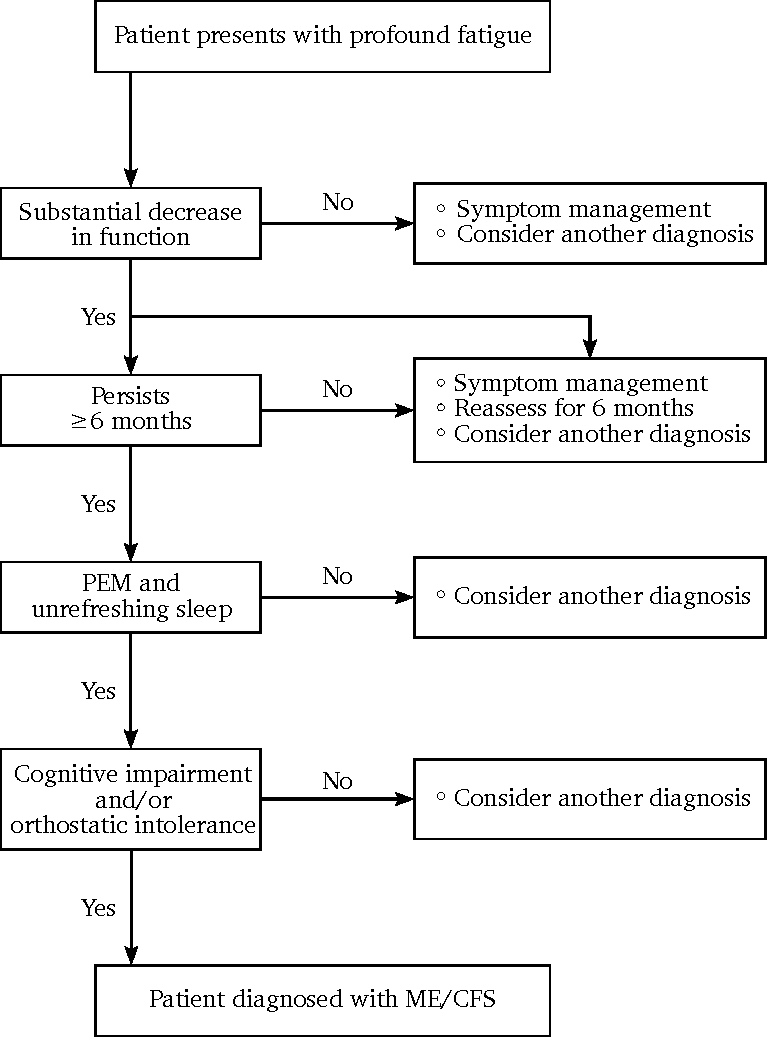
\includegraphics[width=0.75\textwidth]{chapter/introduction/figures/iom-diagnosis-tikz.pdf}
    \caption[Example of a diagnostic flowchart for ME/CFS]{Example of a diagnostic flowchart for ME/CFS. Source: \citet[chap.~7]{instituteofmedicine2015MyalgicEncephalomyelitis}. PEM, post-exertional malaise.}
    \label{fig:intro-flowchart}
\end{figure}
% Figure 1
% Figure~\ref{fig:intro-flowchart}

The definitions more widely used are the Fukuda/CDC (CDC-1994, \citealt{fukuda1994ChronicFatigue}), the Canada Consensus Criteria (CCC-2003, \citealt{carruthers2003MyalgicEncephalomyelitis}), the International Consensus Criteria (ICC-2011, \citealt{carruthers2011MyalgicEncephalomyelitis}), and the Institute of Medicine Criteria (IOM-2015, \citealt{instituteofmedicine2015MyalgicEncephalomyelitis}). These criteria will be further discussed in \textbf{Chapter~\ref{chapter:statical-challenges-2021}}.

Briefly, the CDC-1994 requires a patient to display unexplained, persistent, or relapsing fatigue for at least six months, accompanied by at least four of eight additional fatigue-related symptoms \citep{fukuda1994ChronicFatigue}.
% The required symptoms are (1) impaired memory or concentration, (2) sore throat, (3) tender cervical or axillary lymph nodes, (4) muscle pain, (5) joint pain, (6) headache, (7) unrefreshing sleep and (8) post-exertional malaise (post-exertional malaise)
The CCC-2003 requires a minimum of four fatigue-specific symptoms, at least two neurological or cognitive symptoms, and at least one manifestation from the autonomic, neuroendocrine, or immune domain \citep{carruthers2003MyalgicEncephalomyelitis}.
% interestingly, depression in listed here as a comorbidity of ME/CFS.
The ICC-2011 is a modification of the previous CCC-2003 and focuses less on the prolonged and persistent characteristics of fatigue. Individuals are diagnosed if fatigue results in at least a 50\% reduction of their pre-morbid activity levels. Additionally, post-exertional neuro-immune exhaustion (equivalent to post-exertional malaise), at least one neurological symptom, at least one immune, gastro-intestinal, or genitourinary symptom, and at least one symptom related to energy production/transportation are required \citep{carruthers2011MyalgicEncephalomyelitis}.
% i.e., physical or cognitive fatigue as response to minimal exertion, can be immediate or delayed, and takes longer than 24 hours to recover from it while exacerbating the other symptoms; broadly 
% This is described as physical and/or cognitive fatigue in response to minimal exertion, which can be immediate or delayed, takes longer than 24 hours to recover from and causes ME symptom exacerbation.
% Patients must also present with at least one of the following neurological impairment symptoms; difficulty processing information, short-term memory loss, headaches, significant musculoskeletal pain, disturbed sleep patterns, unrefreshing sleep, sensory sensitivity or paresis.
% Patients must also present with at least one immune (e.g. flu-like symptoms), GI (e.g. irritable bowel syndrome (IBS)) or GU (e.g. altered urinary urgency) symptom.
% Finally, patients must have at least one of the following energy production impairments; orthostatic intolerance, hypotension, postural orthostatic tachycardia syndrome (POTS), palpitations, light-headedness, laboured breathing, fatigue of chest wall muscles, feeling feverish, cold extremities and intolerance of extreme temperatures.
The IOM-2015 was developed as a primary diagnostic tool for clinical purposes. It focuses on specific symptoms impacting the patient's pre-illness activity levels and causing distressing levels of cognitive impairment and/or orthostatic intolerance \citep{instituteofmedicine2015MyalgicEncephalomyelitis}.

% \note{Exclusion factors}
Exclusionary conditions typically include active medical conditions or disease processes that could explain the major symptoms of fatigue, psychiatric disorders, major depressive disorder, substance abuse, severe obesity or eating disorders, and chronic viral infections. However, exclusionary conditions also vary between case criteria, and efforts have been made to standardise the selected conditions across studies \citep{jason2023EstablishingConsensus}.
% It is worth noting that widespread fatigue is a common manifestation in various diseases (and even in healthy individuals).

% \note{Impact}
The lack of consistency across case definitions (in both inclusion and exclusion criteria) poses a major challenge in ME/CFS research \citep{jason2014ExaminingCase, nacul2017DifferingCase}. The heterogeneity seen in patient cohorts, from the multiplicity of symptoms and use of different case definitions, inevitably contributes to the lack of replication observed in studies and hinders the identification of biomarkers and effective treatments \citep{nacul2019HowHave, malato2021Statisticalchallenges, malato2023ImpactMisdiagnosis}. Moreover, ME/CFS might also represent a spectrum of diseases with similar clinical symptoms but potentially diverse mechanisms and pathways \citep{jason2005ChronicFatigue}. These factors contribute to delays and possible misdiagnosis of patients, and it is expected that there is still a large number of non-diagnosed cases \citep{solomon2004FactorsInfluencing, bayliss2014OvercomingBarriers}.
% Moreover, ME/CFS could simply be an umbrella term that characterises a wide spectrum of diseases---or even low-graded diseases---all exhibiting similar clinical symptoms despite potentially having different mechanisms and pathways \citep{jason2005ChronicFatigue}.

% % \note{Silver lining}
% In recent years, clinicians and researchers have coordinated efforts to define a standardised clinical diagnosis for ME/CFS for clinical and research use \citep{nacul2021EuropeanNetwork}, with emphasis on the evaluation of diagnostic criteria through appropriate questionnaires, coupled with a comprehensive medical history, physical examination, functional tests and analyses, and with appropriate differential diagnostics \citep{pheby2020DevelopmentConsistent, steiner2023UnderstandingDiagnosing}. The reduction in ambiguity in disease definition ensures more consistent results in both the diagnosis and sampled cohorts used in research \citep{scheibenbogen2017EuropeanME}.
% \red {improve closing paragraph or change it to research challenges?}

% Physical tests
%     1. Checklist Individual Strenght, for fatigue severity
%     2. Sickness Impact Profile-8, for functional impairment
%     3. Short Form-36, for physical functioning
%     Other proposals: DePaul questionnaire \citep{jason2018DevelopmentDePaul}
%     - DAS-28
% important papers:    
%     - UKMEB \citep{lacerda2018UKME, lacerda2017UKME}
%     - \citep{scheibenbogen2017EuropeanME}
% ME/CFS symptoms and risk factors
%     - photophobia \citep{cortese2018PhotophobiaMultiple}
%     - PEM \citep{chu2018DeconstructingPostexertional}
%     - sleep patterns \citep{jain2017PrevalenceRisk}
%     - stress https://onlinelibrary.wiley.com/doi/10.1002/9781118993811.ch8
%     - pathophysiological mechanisms \citep{lorussoImmunologicalAspectsChronic2009}:
%         - Altered central nervous system functioning resulting from an abnormal immune response against a common antigen
%         - Neuroendocrine disturbance
%         - Cognitive impairment caused by response to infection or other stimuli in sentient people
%     - como é realizado o diagnóstico
%         - múltiplos diagnósticos
%             - 25 case definitions \citep{lim2020ReviewCase}
%             - citar outros
%%%%%%%%%%%%%%%%%%%%%%%%%%%%%%%%%%%%%%%%%%%%%%%%%%%%%%%%%%%%%%%%%%%%%%%%
%%%%%%%%%%%%%%%%%%%%%%%%%%%%%%%%%%%%%%%%%%%%%%%%%%%%%%%%%%%%%%%%%%%%%%%%
% \subsection{Similarities to other diseases}
\subsection{Connection to other diseases}
\label{subsec:similatities-other-diseases}
% \subsection{Similar and co-morbid diseases}

% \note{Intro}
When investigating pathophysiological pathways or potential disease biomarkers in \cfs, many studies commonly include matched healthy individuals as the control group (some of them self-reported participants).
Conversely, the comparison with other fatigue-inducing diseases has also proven to be of value.
Firstly, biologically identifiable diseases, such as cancer or type 1 diabetes, can serve as exclusionary factors in the diagnosis for \cfs \citep{carruthers2003MyalgicEncephalomyelitis}.
Secondly, exploring associations with other post-infectious and autoimmune diseases of uncertain aetiology can be essential in understanding how to better characterise \cfs and its origin, helping to improve diagnosis or treatment strategies.
% since there is considerable overlap between symptoms assessed \citep{malato2021Statisticalchallenges, domingues2023AssociationAnalysis}.
% \citep{almenar-perez2020AssessingDiagnostic, bertinat2022DecreasedNO, blauensteiner2021AlteredEndothelial, gonzalez-cebrian2022DiagnosisMyalgic}


% \note{MS}
% One of the extensively compared diseases is m
Multiple sclerosis (MS) is commonly included as disease control in \cfs studies.
It is an autoimmune condition characterised by the involvement of auto-reactive T and potentially B cells against brain and spinal cord antigens.
This results in the formation of sclerotic plaques in the brain and spinal cord, leading to the destruction of myelin sheaths surrounding nerve cell axons and causing symptoms such as muscle weakness and ataxia \citep{janeway2017Immunology, dobson2019MultipleSclerosis}.
Although there are associations with post-acute infections caused by herpesviruses such as EBV \citep{wang2020HLADR15Molecules, bjornevik2022LongitudinalAnalysis} and HHV6 \citep{engdahl2019IncreasedSerological}, the exact pathway leading to MS remains unknown \citep{sedighi2022ComprehensiveInvestigations}.

% \note{MS and ME/CFS}
MS patients exhibit symptoms overlapping with those of \cfs, including chronic and disabling fatigue, autonomic, and neurocognitive symptoms \citep{morrisMyalgicEncephalomyelitisChronic2013, gaberMultipleSclerosisChronic2014}.
However, there are distinct symptomatological patterns able to differentiate between the two conditions \citep{jasonDifferentiatingMultipleSclerosis2017, domingues2023AssociationAnalysis}.
Notably, a study reported that tender lymph nodes and flu-like symptoms could differentiate MS and \cfs individuals with an accuracy of approximately 81\% \citep{ohanian2016IdentifyingKey}.
MS also serves as direct control in \cfs studies assessing the autoimmune hypothesis, with extensive literature exploring various disease pathways \citep{ramosRegulatoryNaturalKiller2016, jain2017PrevalenceRisk, cliff2019CellularImmune, melvin2019CirculatingLevels, lacerda2019HopeDisappointment}.
For instance, \citet{cliff2019CellularImmune} compared \cfs subgroups with MS and found significant differences in immune-cell populations, including increased monocytes, dendritic cells, and \cdfour T cells, and decreased \cdeight T cells, which in turn were not observed when compared with healthy controls.
% In another example, there are findings supporting comparable mean stress-related growth/differentiation factor 15 peptide levels in both the MS and ME/CFS groups \citep{melvin2019CirculatingLevels}.

Large biobanks specialised in \cfs, such as the United Kingdom ME/CFS biobank (UKMEB), have incorporated MS patients as a disease control group \citep{lacerda2017UKME, lacerda2018UKME}.
Moreover, when possible, control data from MS patients were included in the analyses throughout this thesis, including symptoms (\textbf{Chapter~\ref{chapter:statical-challenges-2021}} and \textbf{Chapter~\ref{chapter:2023-sym-and-herpesvirus}}) and antibody concentrations (\textbf{Chapter~\ref{chapter:2023-sym-and-herpesvirus}}).

% Research on the aetiological hypothesis of autoimmunity for ME/CFS should then focus on studying possible causing mechanisms while identifying the main differences between what is found in ME/CFS and other different and known autoimmune diseases.

% - \red{\citet{brenu2014RoleAdaptive} proposes that ME/CFS patients have a similar pattern of B cell distribution seen in both MS, RA and SLE.}
% - \citep{ramosRegulatoryNaturalKiller2016} fail to identify common immunological disturbances between both diseases.
% - However, there is evidence suggesting different pathways of disease.

% - which make this disease distinct from ME/CFS. However, as a complex autoimmune disease with many associated genetic loci, people with MS are usually included as controls in studies (example, used in Chapter \ref{chapter:statical-challenges-2021} and Chapter \ref{chapter:2023-sym-and-herpesvirus}).
% Assessing the multitude of possible pathogenesis, when searching for possible disease markers, most studies compare diagnosed ME/CFS individuals to a cohort of matched healthy controls (some of them also self-reported members from staff) \citep{almenar-perez2020AssessingDiagnostic, bertinat2022DecreasedNO, blauensteiner2021AlteredEndothelial, gonzalez-cebrian2022DiagnosisMyalgic}.
% However, the use of other similar diseases as controls could also be important (e.g., \citet{ramosRegulatoryNaturalKiller2016, cliff2019CellularImmune, jain2017PrevalenceRisk, lacerda2019HopeDisappointment, melvin2019CirculatingLevels}.

% infectious diseases,  and multiple autoimmune disorders.
% - doenças usadas como comparadores
% - sintomas semelhantes e overlapping

%%%%%%%%%%%%%%%%%%%%%%%%%%%%%%%%%%%%%%%%%%%%%%%%%%%%%%%%%%%%%%%%%%%%%%%%
% \subsubsection{Multiple sclerosis (MS)}
% - ME/CFS vs MS studies \citep{loebel2017SerologicalProfiling, ramosRegulatoryNaturalKiller2016}
% - similarities between symptoms: share neurological symptoms, such as bran fog, memory loss, cognitive impairment, and photosensitivity/photophobia \citep{morrisMyalgicEncephalomyelitisChronic2013}
% - differences between symptoms: ME/CFS have more symptoms and with higher severity \citep{jasonDifferentiatingMultipleSclerosis2017, domingues2023AssociationAnalysis}
% - unknown exact pathway that leads to MS
% - many genes have been associated with the disease dobson2019MultipleSclerosis.
% - immune comparison between ME/CFS and MS \citep{ramosRegulatoryNaturalKiller2016} -- MS was deemed a an important control given that patients afflicted with this disease experience chronic fatigue as major manifestation.
% - Also they share neurological symptoms (brain fog, memory loss, cognitive impairment, photosensibility/photophobia) \citep{morrisMyalgicEncephalomyelitisChronic2013}
% - Large specialised biobanks such as the UKMEB have included MS patients to be used as disease control group. For this purpose, data from MS patients was analysed when possible throughout this thesis. Namely MS patients symptoms (Chapter~\ref{chapter:statical-challenges-2021} and Chapter~\ref{chapter:2023-sym-and-herpesvirus}) and antibody concentrations (Chapter~\ref{chapter:2023-sym-and-herpesvirus}).

%%%%%%%%%%%%%%%%%%%%%%%%%%%%%%%%%%%%%%%%%%%%%%%%%%%%%%%%%%%%%%%%%%%%%%%%
% \subsubsection{Fibromyalgia (FM)}
% \note{FM}
Similar to MS, fibromyalgia (FM) shares a considerable number of symptoms with \cfs, including persistent fatigue, widespread pain and sensitivity, cognitive dysfunction, and sleep problems.
FM also encompasses a heterogeneous population, characterised by heightened central sensitivity to peripheral sensations
\citep{kodner2015CommonQuestions}.
Interestingly, there are no medical exclusions in the diagnosis of FM.
Instead, patients are diagnosed as having primary or secondary FM, mainly depending on whether their symptoms are unique or co-exist with other rheumatological diagnoses, respectively \citep{natelsonMyalgicEncephalomyelitisChronic2019}.

% \note{FM and ME/CFS}
The overlap between FM and \cfs has even led to discussions about whether the two illnesses represent distinct expressions of the same syndrome, and studies have analysed their differences \citep{abbiChronicFatigueSyndrome2012, castro-marrero2013CouldMitochondrial}.
For example, \citet{vegaDNAMethylationModifications2014} found a pattern of epigenetic modifications in \cfs related to immune response and discussed the possible biological difference between the two conditions by highlighting that epigenomic analyses in FM patients found differential methylation of genes associated with structural and nervous system development and neuron differentiation instead.
Another key difference is that physical activity in FM patients can lead to positive outcomes and alleviate the experienced symptoms of pain, whereas in \cfs patients, exercise worsens PEM and related symptoms \citep{hauser2010EfficacyDifferent, kodner2015CommonQuestions}.
% - Changes in neurotransmitter systems can affect, for example, pain-processing networks, modulation of sensory input and cognition. Such mechanisms have been suggested to play a role in fibromyalgia [33] and may possibly also come into play in the development of CFS/ME \citep{foerster2012ReducedInsular}.


% \note{Other diseases}
Other overlapping illnesses are studied alongside research in \cfs.
Examples include rheumatoid arthritis \citep{moss-morris2003IllnessPerceptions, davis2008ChronicStressa, ali2017FatiguePsychosocial}, Sj\"{o}gren's syndrome \citep{calabrese1994ChronicFatigue, kim2023CharacterizingSjogrenAssociated}, Gulf War syndrome \citep{kang2003PosttraumaticStress, halpin2017MyalgicEncephalomyelitis}, systemic lupus erythematosus \citep{sotznyMyalgicEncephalomyelitisChronic2018}, and Long Covid \citep{komaroff2023MECFS, gil2023IdentificationCD8}, among others.% (Table~\ref{tab:intro-similar-diseases}).
Notably, these and other diseases share a link to post-acute infection sequelae \citep{choutka2022UnexplainedPostacute}.
Associations between the latter condition and \cfs will be briefly discussed later in the thesis (\textbf{Chapter~\ref{chapter:discussion}}).

% \subsubsection{Rheumatoid arthritis (RA)}    
% - Elevation of pro-inflammatory cytokine IL-6 in mononuclear cells from fatigued patients with RA (https://www.ncbi.nlm.nih.gov/pmc/articles/PMC2211450/)
% - correlated fatigue with depression and anxiety (https://pubmed.ncbi.nlm.nih.gov/20007746/)
% - DAS-28 reports worse results in RA patients in tender joints, swollen joints, pain scores, and general health rating

% \begin{table}[htbp]
%     \centering
%     \caption{List of diseases similar/overlapping with ME/CFS.}
%     % % \begin{tabular}{@{}lll@{}}
% \toprule
% Stratification & Considerations & Examples of references \\
% \midrule
% \begin{tabular}[c]{@{}l@{}}Presence/severity\\of symptoms \end{tabular} & 
%     \begin{tabular}[c]{@{}l@{}}Absent--Mild vs. Moderate--Severe \end{tabular} & 
%     \begin{tabular}[c]{@{}l@{}}
%         \citet{cliff2019CellularImmune}
%     \end{tabular} \\
%  & & \\
% \begin{tabular}[c]{@{}l@{}}Groups/subgroups\\of specific symptoms \end{tabular} & 
%     \begin{tabular}[c]{@{}l@{}}Identification of cluster\\from specific domains (Table~\ref{tab:intro-symptom-domains}) \end{tabular} & 
%     \begin{tabular}[c]{@{}l@{}}
%         \citet{asprustenAreThereSubgroups2021};\\
%         \citet{malato2021Statisticalchallenges};\\
%         \textcolor{red}{Chapter}~\ref{}\\
%     \end{tabular} \\
%  & & \\
% \begin{tabular}[c]{@{}l@{}}Infection trigger/\\ viral infection \end{tabular} & 
%     \begin{tabular}[c]{@{}l@{}}Link with (auto)immune dysregulations\\ (Unknown/No, Yes/Yes confirmed in laboratory)\end{tabular} & 
%         \begin{tabular}[c]{@{}l@{}}
%             \citet{domingues2021HerpesvirusesSerologya};\\ 
%             \citet{ruiz-pablos2021EpsteinBarrVirus};\\ 
%             \citet{sepulveda2022RevisitingIgG}
%         \end{tabular} \\
%  & & \\
% \begin{tabular}[c]{@{}l@{}}Duration of illness \end{tabular} & 
%     \begin{tabular}[c]{@{}l@{}}Self-assessment of disease;\\Disease progression stage \end{tabular} & 
%     \begin{tabular}[c]{@{}l@{}}
%         \citet{brenu2012LongitudinalInvestigation}
%     \end{tabular} \\
%  & & \\
% \begin{tabular}[c]{@{}l@{}}Illness onset \end{tabular} & 
%     \begin{tabular}[c]{@{}l@{}}Gradual vs. sudden stage \end{tabular} & 
%     \begin{tabular}[c]{@{}l@{}}. \end{tabular} \\
%  & & \\
% \begin{tabular}[c]{@{}l@{}}Age \end{tabular} & 
%     \begin{tabular}[c]{@{}l@{}}. \end{tabular} & 
%     \begin{tabular}[c]{@{}l@{}}
%     \end{tabular} \\
%  & & \\
% \begin{tabular}[c]{@{}l@{}}Comorbidities \end{tabular} & 
%     \begin{tabular}[c]{@{}l@{}}Possible predispositions such as associated\\family diseases \end{tabular} & 
%     \begin{tabular}[c]{@{}l@{}}\citet{lacerdaLogisticRegressionAnalysis2019}\end{tabular} \\
%  & & \\
% \begin{tabular}[c]{@{}l@{}}Multiple phenomena \end{tabular} & 
%     \begin{tabular}[c]{@{}l@{}}. \end{tabular} & 
%     \begin{tabular}[c]{@{}l@{}}\citet{asprustenAreThereSubgroups2021} \end{tabular} \\
%  & & \\
% \begin{tabular}[c]{@{}l@{}}Response to treatments \end{tabular} & 
%     \begin{tabular}[c]{@{}l@{}}. \end{tabular} & 
%     \begin{tabular}[c]{@{}l@{}} \end{tabular} \\
%  & & \\
% \begin{tabular}[c]{@{}l@{}}. \end{tabular} & 
%     \begin{tabular}[c]{@{}l@{}}. \end{tabular} & 
%     \begin{tabular}[c]{@{}l@{}}. \end{tabular} \\
% \bottomrule
% \end{tabular}
\begin{tabular}[c]{m{0.25\textwidth} m{0.5\textwidth} m{0.25\textwidth}}
\toprule
Stratification & Considerations & Examples of references \\
\midrule
\begin{tabular}[c]{@{}l@{}}Presence/severity\\of symptoms\end{tabular} & Compare subgroups for Absent vs. Present or Absent--Mild vs. Moderate--Severe & \begin{tabular}[c]{@{}l@{}}\citet{landay1991ChronicFatigue};\\ \citet{hardcastle2014AnalysisRelationship};\\
\citet{montoyaCytokineSignatureAssociated2017};\\
\citet{cliff2019CellularImmune}\end{tabular}\\
 & & \\
\begin{tabular}[c]{@{}l@{}}Subgroups of symptoms\end{tabular} & Identification of similar clusters within specific domains (Table~\ref{tab:intro-symptom-domains}) &
\begin{tabular}[c]{@{}l@{}}\citet{asprustenAreThereSubgroups2021};\\ Chapter~\ref{chapter:2024-sym-domains} \end{tabular}\\
 & & \\
\begin{tabular}[c]{@{}l@{}}Disease onset/trigger\end{tabular} & Link with (auto)immune dysregulations and production of autoantibodies; Unknown/No infection vs. Infection & 
\begin{tabular}[c]{@{}l@{}}\citet{szklarski2021DelineatingAssociationa};\\ \citet{domingues2021HerpesvirusesSerologya};\\ \citet{ruiz-pablos2021EpsteinBarrVirus};\\ \citet{sepulveda2022RevisitingIgG}\end{tabular}\\
& & \\
Disease duration & Linked with disease progression stages; Prodormal vs. Early vs. Established disease & \begin{tabular}[c]{@{}l@{}}\citet{brenu2012LongitudinalInvestigation};\\ \citet{stoothoffSubtypingPatientsMyalgic2017};\\ \citet{nacul2020HowMyalgic}\end{tabular} \\
& & \\
Age & Differences in severity of experienced symptoms & \begin{tabular}[c]{@{}l@{}}\citet{itoh2012FibromyalgiaChronic};\\ \citet{lewis2013ChronicFatigue};\\ \citet{miike2008ChronicFatigue}\end{tabular}\\
& & \\
Sex & Hormonal differences and possible predisposition towards the disease & \citep{pipper2023SexDisease} \\
% & & \\
% Comorbidities & Possible predispositions; linked with demographics and/or family history & \citet[Box~8]{nacul2021EuropeanNetwork} \\
% & & \\
% Treatments & Differences in response to treatments (clinical trials) or therapies & \citet{flugeBLymphocyteDepletionPatients2019} \\
% & & \\
% Multiple phenomena &  &  \\
% & & \\
\bottomrule
\end{tabular}
% \begin{tabular}[c]{@{}l@{}}  \end{tabular}



%     \resizebox{\textwidth}{!}{\begin{tabular}[c]{m{0.3\textwidth} m{0.45\textwidth} m{0.25\textwidth}}
\toprule
Illness & Short description and overlap & References on the two \\
\midrule
Multiple sclerosis & & \\
& & \\
Fibromyalgia& & \\
& & \\
Rheumatoid arthritis& & \citet{davis2008ChronicStressa, ali2017FatiguePsychosocial}\\
& & \\
Sj\"{o}gren's syndrome& & \citet{calabrese1994ChronicFatigue, kim2023CharacterizingSjogrenAssociated}\\
& & \\
Gulf War syndrome& & \citet{kang2003PosttraumaticStress}\\
& & \\
Long Covid& & \\
& & \\
Postural tachycardia syndrome& & \\
& & \\
Inflammatory bowel syndrome& & \citet{whitehead2002SystematicReview}\\
& & \\
Systemic lupus erythematosus& & \\
& & \\
Autoimmune (Auto-inflammatory) syndrome induced by adjuvants& & \\
& & \\
Crohn’s disease& & \\
& & \\
Hashimoto's thyroiditis& & \\
& & \\
Major depressive disorder& & \\
% & & \\
\bottomrule
\end{tabular}
% \begin{tabular}[c]{@{}l@{}}  \end{tabular}


}
%     \label{tab:intro-similar-diseases}
% \end{table}
% % Table~\ref{tab:intro-similar-diseases}

% \begin{itemize}
%     \setlength{\itemsep}{1.5pt}
%     \setlength{\parskip}{0pt}
%     \setlength{\parsep}{0pt}
%     \item Sj\"{o}gren's syndrome (SS)
%     \item Gulf War syndrome/illness (GWS): exposição a quimicos (mutação genética em alguns soldados?) Não metabolizam e libertam toxinas (vacinação massiva e exposição a quimicos)
%     \item Postural tachycardia syndrome (POTS)
%     \item Inflammatory bowel disease (IBS): Factors mostly linked with chronic fatigue: haemoglobin values, present gastrointestinal symptoms, and altered sleep (https://pubmed.ncbi.nlm.nih.gov/21674713/)
%     \item Systemic lupus erythematosus (SLE)
%     \item Chronic obstructive pulmonary disease
%     \item Autoimmune (Auto-inflammatory) Syndrome induced by Adjuvants (ASIA)
%     \item Crohn's disease (CD)
%     \item Hashimoto's thyroiditis: perforin is low in patients (https://www.ncbi.nlm.nih.gov/pmc/articles/PMC4439970/)
%     \item Other less direct diseases:
%     \begin{itemize}
%         \item Major depressive disorder (MDD)
%         \item Some neurologic disorders (i.e., stroke)
%         \item Cancer
%     \end{itemize}
% \end{itemize}


%%%%%%%%%%%%%%%%%%%%%%%%%%%%%%%%%%%%%%%%%%%%%%%%%%%%%%%%%%%%%%%%%%%%%%%%
%%%%%%%%%%%%%%%%%%%%%%%%%%%%%%%%%%%%%%%%%%%%%%%%%%%%%%%%%%%%%%%%%%%%%%%%
\subsection{Treatment and prognosis}
\label{subsec:treatment-prognosis}

% \note{Treatment}
As of now, there is no known cure or approved treatment for ME/CFS.
Clinical support mostly focuses on accommodation and symptom management, assisting patients in understanding how to cope with the disease and strike a balance between rest and activity to prevent the worsening of their symptoms \citep{carruthers2003MyalgicEncephalomyelitis, rowe2017MyalgicEncephalomyelitis}.
Educating the patients and their support networks about the illness can be important in fostering a sense of control over the symptoms, which has shown to be a positive long-term outcome \citep{cairns2005SystematicReview}.
% capacitating patients with a sense of control has shown to be a positive indicator and yielded an improvement in the long-term outcome is the capacitation of \cfs patients with a sense of control over their symptoms \citep{cairns2005SystematicReview}.

The primary symptoms targeted include PEM, unrefreshing sleep and sleep habits, pain and discomfort in muscles and joints, headaches, dizziness or orthostatic intolerance, and memory and concentration problems.
While anti-viral therapies and treatments for immune dysfunction, hypothalamic-pituitary-adrenal axis abnormalities, and autonomic or central nervous system dysfunction may be considered, their efficacy remains uncertain \citep{carruthers2003MyalgicEncephalomyelitis}.
Alternatively, non-pharmacological interventions and medications may also be prescribed for the treatment and management of symptoms \citep{rowe2017MyalgicEncephalomyelitis}.
However, ME/CFS often exhibit hypersensitivity to standard medications given in the usual doses and can experience side effects or worsened symptoms.
Being a heterogeneous group, prescribed medication that works for some can worsen the experienced symptoms in others \citep{carruthers2003MyalgicEncephalomyelitis}.
% usually sleep disturbance, pain, fatigue and PEM, cognitive dysfunctions

In addition to symptom management, lifestyle adjustments and self-help therapies are also focused in \cfs.
While adjusting to the disease, patients may experience co-occurring conditions such as depression, stress, and anxiety states, which can be addressed through supportive counselling and medical recommendations.
Ultimately, while both direct actions on specific symptoms and overall patient well-being can provide some relief and improve quality of life, the approaches are very case-dependent, and treatment programs are recommended to be individualised, with regular assessments to monitor progress and watch for the possible emergence of other illnesses.

% \note{Prognosis}
The long-term prognosis for ME/CFS remains uncertain and varies among individuals. 
While some studies suggest better outcomes with older age \citep{ghali2022FactorsInfluencing}, the general trend is the reduction or improvement of symptoms rather than full recovery \citep{carruthers2011MyalgicEncephalomyelitis, nacul2021EuropeanNetwork}.

% Full recovery is not the norm and the general reduction or improvement of symptoms is commonly reported 
% % The median duration \citep{reynolds2004EconomicImpact}
% \textcolor{red}{(Should talk about long term prognosis and recovery times? \citep{carruthers2011MyalgicEncephalomyelitis, rowe2017MyalgicEncephalomyelitis})}
% % time of disease
% \citep{slomko2019PrevalenceCharacteristics}

% - B cell depletion: \citep{flugeBLymphocyteDepletionPatients2019}

\red{Should provide examples of proposed treatments (PACE trial, rituximab, valacyclovir)? Examples: \citep{lerner2007ValacyclovirTreatment, white2011ComparisonAdaptivea, montoya2013RandomizedClinical, diaz-mitoma2003ClinicalImprovement}, and problems \citep{geraghty2017PACEGateWhen}}

% \subsubsection{Examples of proposed treatments?}
% - six-month treatment of ME/CFS seropositive for EBV with valacyclovir---antiviral drug---improved their physical functional capacity with improvements in cardiac function \citep{lerner2007ValacyclovirTreatment}
% - six-month trial with valganciclovir---antiviral drug (another)---had positive results in another cohort of ME/CFS patients \citep{montoya2013RandomizedClinical}
% - isoprinosine---another antiviral that amplifies the natural immune response---increased NK cell activity and IL-12 production in a cohort of patients, with improvement in the overall health measurements \citep{diaz-mitoma2003ClinicalImprovement}.

% Another study reported that individuals with ME/CFS exhibited impaired endothelial function compared to healthy controls, as evidenced by reduced flow-mediated dilation, a measure of endothelial function \citep{sorland2021ReducedEndothelial}. The same study proposed treatment with cyclophosphamide, but the results did not show endothelial function improvement after intervention \citep{sorland2021ReducedEndothelial}.



%%%%%%%%%%%%%%%%%%%%%%%%%%%%%%%%%%%%%%%%%%%%%%%%%%%%%%%%%%%%%%%%%%%%%%%%
%%%%%%%%%%%%%%%%%%%%%%%%%%%%%%%%%%%%%%%%%%%%%%%%%%%%%%%%%%%%%%%%%%%%%%%%
% \section{Key biological questions and shortcomings to the disease study}
% - lack of progress \citep{luis_nacul_how_2020}


%%%%%%%%%%%%%%%%%%%%%%%%%%%%%%%%%%%%%%%%%%%%%%%%%%%%%%%%%%%%%%%%%%%%%%%%
%%%%%%%%%%%%%%%%%%%%%%%%%%%%%%%%%%%%%%%%%%%%%%%%%%%%%%%%%%%%%%%%%%%%%%%%
\subsection{Research challenges}
\label{subsec:research-challenges}

% \note{complex aetiology}
% \note{symptom heterogeneity}
% \note{no biomarker}
% \note{overlap with other conditions}
% \note{limited understanding of pathophysiology}
% \note{reduced treatment options}
% \note{patient stratification}
% \note{stigma and misconception}
% \note{limited longitudinal studies on the natural progression of ME/CFS}

% symptom heterogeneity
ME/CFS has a complex aetiology and multifactorial nature, with signals of involvement from immune dysregulation, genetic/epigenetic predisposition, environmental factors, and potential viral infections \citep{rivera2019MyalgicEncephalomyelitis}.
This diversity of influencing factors contributes to the ample heterogeneity of observed symptoms and severities, often overlapping with diseases of complex diagnosis, ultimately posing a challenge to the understanding of what the underlying causes may be \citep{malato2021Statisticalchallenges}.

% lack of diagnosis consensus
The lack of consensus on disease definition also generates uncertainty, as illustrated by the lack of consistency in findings across various fields of research (\textbf{Section~\ref{subsec:pathogenesis}}).
Moreover, limited funding for research on ME/CFS hinders the ability to develop large-scale longitudinal study designs with large sample sizes, leading to a lack of statistical power to test hypotheses and validate potential associations found \citep{malato2022ImpactMisclassification}.
% Burden and funding
A study in the US estimated that ME/CFS poses an economic burden of 36 to 51 billion dollars annually \citep{jason2021UpdatingNational}, and studies in Europe propose similar values, adding that a modest 1\% reduction in the overall burden of ME/CFS could deliver annual cost savings of approximately 400 million euros \citep{mccrone2003EconomicCost, pheby2020DevelopmentConsistent}, putting it on par and even surpassing comparable diseases.
Yet, ME/CFS receives comparatively less research funding \citep{mirin2022UpdatedME}.
Additionally, the use of self-reported cases---in both patients and, at times, healthy controls---is also a problem.
A Polish study assessing the prevalence and characteristics of ME/CFS in a community identified 1400 individuals who were believed to be suffering from ME/CFS, but only 69 individuals actually complied with a case definition \citep{slomko2019PrevalenceCharacteristics}.
% Another study had a patient initially diagnosed with ME/CFS but later was found to have a rare autosomal adult-onset disorder \citep{brown2021MECFS}.

From the overall uncertainty surrounding this disease, one additional reason for lack of consensus and resulting number of contrasting evidence could be the misdiagnosis of patients \citep{nacul2019HowHave}.
Misdiagnosis can arise from the lack of agreement between case definitions, by diagnosing distinct suspected cases \citep{nacul2017DifferingCase, malato2021Statisticalchallenges}, or when failing to diagnose other overlapping diseases \citep{nacul2019HowHave, malato2023ImpactMisdiagnosis}, and several works have proposed the stratification of ME/CFS into specific subgroups as a way to minimise this transversal effect (Table~\ref{tab:intro-stratification}).
Diagnosed patients can be split by clinically assessed criteria, such as the severity of experienced symptoms, infection as a trigger for the disease, or age \citep{janal2006SubtypingCFS, lewis2013ChronicFatigue, hardcastle2014AnalysisRelationship, domingues2021HerpesvirusesSerologya}.
Alternatively, profiles related to immune and genomic subtypes have also been suggested \citep{kerr2007SevenGenomic, kerr2008GeneExpression, vegaIntegrationDNAMethylation2018}.
% and timely factors such as disease progression could also be linked with functional differences within patients \citep{brenu2012LongitudinalInvestigation}.
Furthermore, timely factors such as disease progression could also be linked with functional differences in ME/CFS, as different patients have shown distinct immune cell dysfunctions over time \citep{maya2023SurveyingMetabolic}.
In this regard, a longitudinal study on cell cytotoxicity and cytokine secretion showed inconsistent levels of cytokines in the same individuals over different timepoints \citep{brenu2012LongitudinalInvestigation}.
Perhaps the identification of immune dysfunctional states (such as anergy, exhaustion, and senescence) within the immune cell populations would help to better understand the disease stage of the patients and help predict disease progression.

% \note{Silver lining}
Ultimately, in recent years, clinicians and researchers have coordinated efforts to define a standardised clinical diagnosis for ME/CFS for clinical and research use \citep{nacul2021EuropeanNetwork}, with emphasis on the evaluation of diagnostic criteria through appropriate questionnaires, coupled with a comprehensive medical history, physical examination, functional tests and analyses, and with appropriate differential diagnostics \citep{pheby2020DevelopmentConsistent, steiner2023UnderstandingDiagnosing}. The reduction in ambiguity in disease definition and stratification of ME/CFS into more homogeneous clusters ensures more consistent results in both the diagnosis and sampled cohorts used in research \citep{scheibenbogen2017EuropeanME}.
\red{improve closing paragraph?}

\begin{table}[h]
    \centering
    \caption{List of suggested proposals for patient stratification.}
    % % \begin{tabular}{@{}lll@{}}
% \toprule
% Stratification & Considerations & Examples of references \\
% \midrule
% \begin{tabular}[c]{@{}l@{}}Presence/severity\\of symptoms \end{tabular} & 
%     \begin{tabular}[c]{@{}l@{}}Absent--Mild vs. Moderate--Severe \end{tabular} & 
%     \begin{tabular}[c]{@{}l@{}}
%         \citet{cliff2019CellularImmune}
%     \end{tabular} \\
%  & & \\
% \begin{tabular}[c]{@{}l@{}}Groups/subgroups\\of specific symptoms \end{tabular} & 
%     \begin{tabular}[c]{@{}l@{}}Identification of cluster\\from specific domains (Table~\ref{tab:intro-symptom-domains}) \end{tabular} & 
%     \begin{tabular}[c]{@{}l@{}}
%         \citet{asprustenAreThereSubgroups2021};\\
%         \citet{malato2021Statisticalchallenges};\\
%         \textcolor{red}{Chapter}~\ref{}\\
%     \end{tabular} \\
%  & & \\
% \begin{tabular}[c]{@{}l@{}}Infection trigger/\\ viral infection \end{tabular} & 
%     \begin{tabular}[c]{@{}l@{}}Link with (auto)immune dysregulations\\ (Unknown/No, Yes/Yes confirmed in laboratory)\end{tabular} & 
%         \begin{tabular}[c]{@{}l@{}}
%             \citet{domingues2021HerpesvirusesSerologya};\\ 
%             \citet{ruiz-pablos2021EpsteinBarrVirus};\\ 
%             \citet{sepulveda2022RevisitingIgG}
%         \end{tabular} \\
%  & & \\
% \begin{tabular}[c]{@{}l@{}}Duration of illness \end{tabular} & 
%     \begin{tabular}[c]{@{}l@{}}Self-assessment of disease;\\Disease progression stage \end{tabular} & 
%     \begin{tabular}[c]{@{}l@{}}
%         \citet{brenu2012LongitudinalInvestigation}
%     \end{tabular} \\
%  & & \\
% \begin{tabular}[c]{@{}l@{}}Illness onset \end{tabular} & 
%     \begin{tabular}[c]{@{}l@{}}Gradual vs. sudden stage \end{tabular} & 
%     \begin{tabular}[c]{@{}l@{}}. \end{tabular} \\
%  & & \\
% \begin{tabular}[c]{@{}l@{}}Age \end{tabular} & 
%     \begin{tabular}[c]{@{}l@{}}. \end{tabular} & 
%     \begin{tabular}[c]{@{}l@{}}
%     \end{tabular} \\
%  & & \\
% \begin{tabular}[c]{@{}l@{}}Comorbidities \end{tabular} & 
%     \begin{tabular}[c]{@{}l@{}}Possible predispositions such as associated\\family diseases \end{tabular} & 
%     \begin{tabular}[c]{@{}l@{}}\citet{lacerdaLogisticRegressionAnalysis2019}\end{tabular} \\
%  & & \\
% \begin{tabular}[c]{@{}l@{}}Multiple phenomena \end{tabular} & 
%     \begin{tabular}[c]{@{}l@{}}. \end{tabular} & 
%     \begin{tabular}[c]{@{}l@{}}\citet{asprustenAreThereSubgroups2021} \end{tabular} \\
%  & & \\
% \begin{tabular}[c]{@{}l@{}}Response to treatments \end{tabular} & 
%     \begin{tabular}[c]{@{}l@{}}. \end{tabular} & 
%     \begin{tabular}[c]{@{}l@{}} \end{tabular} \\
%  & & \\
% \begin{tabular}[c]{@{}l@{}}. \end{tabular} & 
%     \begin{tabular}[c]{@{}l@{}}. \end{tabular} & 
%     \begin{tabular}[c]{@{}l@{}}. \end{tabular} \\
% \bottomrule
% \end{tabular}
\begin{tabular}[c]{m{0.25\textwidth} m{0.5\textwidth} m{0.25\textwidth}}
\toprule
Stratification & Considerations & Examples of references \\
\midrule
\begin{tabular}[c]{@{}l@{}}Presence/severity\\of symptoms\end{tabular} & Compare subgroups for Absent vs. Present or Absent--Mild vs. Moderate--Severe & \begin{tabular}[c]{@{}l@{}}\citet{landay1991ChronicFatigue};\\ \citet{hardcastle2014AnalysisRelationship};\\
\citet{montoyaCytokineSignatureAssociated2017};\\
\citet{cliff2019CellularImmune}\end{tabular}\\
 & & \\
\begin{tabular}[c]{@{}l@{}}Subgroups of symptoms\end{tabular} & Identification of similar clusters within specific domains (Table~\ref{tab:intro-symptom-domains}) &
\begin{tabular}[c]{@{}l@{}}\citet{asprustenAreThereSubgroups2021};\\ Chapter~\ref{chapter:2024-sym-domains} \end{tabular}\\
 & & \\
\begin{tabular}[c]{@{}l@{}}Disease onset/trigger\end{tabular} & Link with (auto)immune dysregulations and production of autoantibodies; Unknown/No infection vs. Infection & 
\begin{tabular}[c]{@{}l@{}}\citet{szklarski2021DelineatingAssociationa};\\ \citet{domingues2021HerpesvirusesSerologya};\\ \citet{ruiz-pablos2021EpsteinBarrVirus};\\ \citet{sepulveda2022RevisitingIgG}\end{tabular}\\
& & \\
Disease duration & Linked with disease progression stages; Prodormal vs. Early vs. Established disease & \begin{tabular}[c]{@{}l@{}}\citet{brenu2012LongitudinalInvestigation};\\ \citet{stoothoffSubtypingPatientsMyalgic2017};\\ \citet{nacul2020HowMyalgic}\end{tabular} \\
& & \\
Age & Differences in severity of experienced symptoms & \begin{tabular}[c]{@{}l@{}}\citet{itoh2012FibromyalgiaChronic};\\ \citet{lewis2013ChronicFatigue};\\ \citet{miike2008ChronicFatigue}\end{tabular}\\
& & \\
Sex & Hormonal differences and possible predisposition towards the disease & \citep{pipper2023SexDisease} \\
% & & \\
% Comorbidities & Possible predispositions; linked with demographics and/or family history & \citet[Box~8]{nacul2021EuropeanNetwork} \\
% & & \\
% Treatments & Differences in response to treatments (clinical trials) or therapies & \citet{flugeBLymphocyteDepletionPatients2019} \\
% & & \\
% Multiple phenomena &  &  \\
% & & \\
\bottomrule
\end{tabular}
% \begin{tabular}[c]{@{}l@{}}  \end{tabular}



    \resizebox{\textwidth}{!}{% \begin{tabular}{@{}lll@{}}
% \toprule
% Stratification & Considerations & Examples of references \\
% \midrule
% \begin{tabular}[c]{@{}l@{}}Presence/severity\\of symptoms \end{tabular} & 
%     \begin{tabular}[c]{@{}l@{}}Absent--Mild vs. Moderate--Severe \end{tabular} & 
%     \begin{tabular}[c]{@{}l@{}}
%         \citet{cliff2019CellularImmune}
%     \end{tabular} \\
%  & & \\
% \begin{tabular}[c]{@{}l@{}}Groups/subgroups\\of specific symptoms \end{tabular} & 
%     \begin{tabular}[c]{@{}l@{}}Identification of cluster\\from specific domains (Table~\ref{tab:intro-symptom-domains}) \end{tabular} & 
%     \begin{tabular}[c]{@{}l@{}}
%         \citet{asprustenAreThereSubgroups2021};\\
%         \citet{malato2021Statisticalchallenges};\\
%         \textcolor{red}{Chapter}~\ref{}\\
%     \end{tabular} \\
%  & & \\
% \begin{tabular}[c]{@{}l@{}}Infection trigger/\\ viral infection \end{tabular} & 
%     \begin{tabular}[c]{@{}l@{}}Link with (auto)immune dysregulations\\ (Unknown/No, Yes/Yes confirmed in laboratory)\end{tabular} & 
%         \begin{tabular}[c]{@{}l@{}}
%             \citet{domingues2021HerpesvirusesSerologya};\\ 
%             \citet{ruiz-pablos2021EpsteinBarrVirus};\\ 
%             \citet{sepulveda2022RevisitingIgG}
%         \end{tabular} \\
%  & & \\
% \begin{tabular}[c]{@{}l@{}}Duration of illness \end{tabular} & 
%     \begin{tabular}[c]{@{}l@{}}Self-assessment of disease;\\Disease progression stage \end{tabular} & 
%     \begin{tabular}[c]{@{}l@{}}
%         \citet{brenu2012LongitudinalInvestigation}
%     \end{tabular} \\
%  & & \\
% \begin{tabular}[c]{@{}l@{}}Illness onset \end{tabular} & 
%     \begin{tabular}[c]{@{}l@{}}Gradual vs. sudden stage \end{tabular} & 
%     \begin{tabular}[c]{@{}l@{}}. \end{tabular} \\
%  & & \\
% \begin{tabular}[c]{@{}l@{}}Age \end{tabular} & 
%     \begin{tabular}[c]{@{}l@{}}. \end{tabular} & 
%     \begin{tabular}[c]{@{}l@{}}
%     \end{tabular} \\
%  & & \\
% \begin{tabular}[c]{@{}l@{}}Comorbidities \end{tabular} & 
%     \begin{tabular}[c]{@{}l@{}}Possible predispositions such as associated\\family diseases \end{tabular} & 
%     \begin{tabular}[c]{@{}l@{}}\citet{lacerdaLogisticRegressionAnalysis2019}\end{tabular} \\
%  & & \\
% \begin{tabular}[c]{@{}l@{}}Multiple phenomena \end{tabular} & 
%     \begin{tabular}[c]{@{}l@{}}. \end{tabular} & 
%     \begin{tabular}[c]{@{}l@{}}\citet{asprustenAreThereSubgroups2021} \end{tabular} \\
%  & & \\
% \begin{tabular}[c]{@{}l@{}}Response to treatments \end{tabular} & 
%     \begin{tabular}[c]{@{}l@{}}. \end{tabular} & 
%     \begin{tabular}[c]{@{}l@{}} \end{tabular} \\
%  & & \\
% \begin{tabular}[c]{@{}l@{}}. \end{tabular} & 
%     \begin{tabular}[c]{@{}l@{}}. \end{tabular} & 
%     \begin{tabular}[c]{@{}l@{}}. \end{tabular} \\
% \bottomrule
% \end{tabular}
\begin{tabular}[c]{m{0.25\textwidth} m{0.5\textwidth} m{0.25\textwidth}}
\toprule
Stratification & Considerations & Examples of references \\
\midrule
\begin{tabular}[c]{@{}l@{}}Presence/severity\\of symptoms\end{tabular} & Compare subgroups for Absent vs. Present or Absent--Mild vs. Moderate--Severe & \begin{tabular}[c]{@{}l@{}}\citet{landay1991ChronicFatigue};\\ \citet{hardcastle2014AnalysisRelationship};\\
\citet{montoyaCytokineSignatureAssociated2017};\\
\citet{cliff2019CellularImmune}\end{tabular}\\
 & & \\
\begin{tabular}[c]{@{}l@{}}Subgroups of symptoms\end{tabular} & Identification of similar clusters within specific domains (Table~\ref{tab:intro-symptom-domains}) &
\begin{tabular}[c]{@{}l@{}}\citet{asprustenAreThereSubgroups2021};\\ Chapter~\ref{chapter:2024-sym-domains} \end{tabular}\\
 & & \\
\begin{tabular}[c]{@{}l@{}}Disease onset/trigger\end{tabular} & Link with (auto)immune dysregulations and production of autoantibodies; Unknown/No infection vs. Infection & 
\begin{tabular}[c]{@{}l@{}}\citet{szklarski2021DelineatingAssociationa};\\ \citet{domingues2021HerpesvirusesSerologya};\\ \citet{ruiz-pablos2021EpsteinBarrVirus};\\ \citet{sepulveda2022RevisitingIgG}\end{tabular}\\
& & \\
Disease duration & Linked with disease progression stages; Prodormal vs. Early vs. Established disease & \begin{tabular}[c]{@{}l@{}}\citet{brenu2012LongitudinalInvestigation};\\ \citet{stoothoffSubtypingPatientsMyalgic2017};\\ \citet{nacul2020HowMyalgic}\end{tabular} \\
& & \\
Age & Differences in severity of experienced symptoms & \begin{tabular}[c]{@{}l@{}}\citet{itoh2012FibromyalgiaChronic};\\ \citet{lewis2013ChronicFatigue};\\ \citet{miike2008ChronicFatigue}\end{tabular}\\
& & \\
Sex & Hormonal differences and possible predisposition towards the disease & \citep{pipper2023SexDisease} \\
% & & \\
% Comorbidities & Possible predispositions; linked with demographics and/or family history & \citet[Box~8]{nacul2021EuropeanNetwork} \\
% & & \\
% Treatments & Differences in response to treatments (clinical trials) or therapies & \citet{flugeBLymphocyteDepletionPatients2019} \\
% & & \\
% Multiple phenomena &  &  \\
% & & \\
\bottomrule
\end{tabular}
% \begin{tabular}[c]{@{}l@{}}  \end{tabular}


}
    \label{tab:intro-stratification}
\end{table}

% Stratifying diagnosed patients into different subtypes \citep{jason2005ChronicFatigue, domingues2021HerpesvirusesSerologya}, or the reduced number of patients recruited in each study \citep{scheibenbogen2017EuropeanME}.
% explain misdiagnosis
% explain patients stratification
% explain low sampling numbers
% - proposed protocols for criteria standardisation \citep{pheby2020DevelopmentConsistent}
% - Measured differences in case-control studies may simply reflect the cumulative effect of multiple small contributions put together \citep{dibble2020GeneticRisk}
% - The behaviour of individuals could also have consequences in the likelihood of the disease, such as a more sedentary lifestyle \citep{dibble2020GeneticRisk}
% - The cells form a complex network of information exchange through a complex web of interactions to reach and maintain a state of homeostasis.
% Relating to disease progression!
% - Implementation of different case criteria can also produce different results. After reporting increased function activation of NK cells \citet{rivasAssociationNKCell2018}
% - High prevalence of herpesviruses in the wider population, and their ablility to establish lifelong infections.
% - Moreover, the difference or simplicity of methods used to quantify antibody concentrations (reduced sensitivity/specificity?) \citep{ariza2020CommentaryAntibodies, domingues2021AnalysisAntibody}.
% - genomic subtypes: kerr2007SevenGenomic
% - (from sepulveda2022RevisitingIgG) \citep{domingues2021HerpesvirusesSerologya}, \citep{sepulveda2022RevisitingIgG} and \citep{steiner2020AutoimmunityRelatedRisk} and \citep{szklarski2021DelineatingAssociationa}: stratification and biomarkers on infection triggered ME/CFS patients; and given the vast number of infectious agents associated with ME/CFS \citep{blomberg2018InfectionEliciteda, rasa2018ChronicViral} this group could be even further stratified based on the nature of the causative infection.

% % microbiome disturbances/intestinal origins of ME/CFS
% - microbiome
%     - alterations in ME/CFS intestinal microbiome
%     - geographical locations affects microbiome biomarkers for ME/CFS
%     - comorbid IBS affects microbiome biomarkers for ME/CFS
%     - neglected components of the intestinal microbiome
% !!- leaky gut (term used to describe the increased permeability of the gut barrier)
%     - evidence of leaky gut in ME/CFS
%     - potential mechanisms
%     - leaky gut and autoimmunity
%     - microbial dysbiosis
% - the gut-brain axis
%     - alterations
    
%         - genetic risk factors
%             - \citep{dibble2020GeneticRisk}
%             - differentialluy regulated immune, metabolic, and neurological functions
%         - endothelial dysfunction
%             - \citep{haffke2022EndothelialDysfunction}
%         - mutisystemic disease
%             - \citep{marks2023ConvergingEvidence}
%         - gut microbiome
%             - \citep{konig2022GutMicrobiome}

% Extensive and well-defined disease definitions are an imperative tool when performing the clinical diagnosis of an individual. Such diagnoses should be recurrently reviewed and updated, as the knowledge on the specific disease grows.

% - dificuldades no diagnóstico \citep{conroy2023EvaluatingCase, jason2015ComparingContrasting, reeves2005ChronicFatigue}
%         - heterogenidade
% efforts were made to investigate empirical approaches to ME/CFS diagnosis \citep{conroy2023EvaluatingCase, jason2015ComparingContrasting, reeves2005ChronicFatigue}.

% - \citet{domingues2021HerpesvirusesSerologya} found reduction in Ab concentrations to EBV in ME/CFS without putative infection trigger and reduction in Ab concentrations to CMV in ME/CFS with confirmed infection trigger

% - Example: Patient initially diagnosed with ME/CFS but was found to have a rare autossomal adult-onset disorder \citep{brown2021MECFS}.

%     - problemas com mau disgnóstico
%         - \citep{nacul2019HowHave}
%         - \citep{nacul2017DifferingCase}
%         - \citep{malato2021Statisticalchallenges}
%         - \citep{malato2022ImpactMisclassification}
%         - self-report assessment instruments
%             - \citep{pheby2021LiteratureReview}
%         - disease definitions
%             - the need for well-designed and statistically powered epidemiological studies \citep{estevez-lopez2020SystematicReviewa}
%             - DePaul questionnaire \citep{jason2018DevelopmentDePaul}
%         - huge possibility for undiagnosis and thus, the disease remais underdiagnosed
%             - undiagnosed patients will receive inapropriate treatment
% Possible stratification methods: 

% - \citep{asprustenAreThereSubgroups2021}
% - There have been proposals for stratification of ME/CFS into more specific groups for a long period now \citep{jason2005ChronicFatigue}. GIVE EXAMPLES OF STRATIFICATION: by severity, infection trigger, immunological profile, ect
% - \citep{stoothoffSubtypingPatientsMyalgic2017}
% - \citep{jonsjoIdentifyingSymptomSubgroups2017}
% - \citep{pendergrastHouseboundNonhouseboundPatients2016}
    
% 1. Severity
% 2. Infection trigger
% 3. sudden vs. gradual onset
% 4. symptom-based domains
% 5. Disease duration
%     - [[Nacul (2020)](https://www.frontiersin.org/articles/10.3389/fneur.2020.00826/full)]
%     - \citep{russell2016IllnessProgression}
% 6. persisteng, incidence, remiting groups, based on the reported illness status \citep{anderson2014QualitativeNatural}

% Initiatives:
% - At the present time, \red{DecodeME} has closed participant recruitment and DNA sample collection.
% - \red{Oslo Chronic Fatigue Consortium}

\clearpage
%%%%%%%%%%%%%%%%%%%%%%%%%%%%%%%%%%%%%%%%%%%%%%%%%%%%%%%%%%%%%%%%%%%%%%%%
%%%%%%%%%%%%%%%%%%%%%%%%%%%%%%%%%%%%%%%%%%%%%%%%%%%%%%%%%%%%%%%%%%%%%%%%
%%%%%%%%%%%%%%%%%%%%%%%%%%%%%%%%%%%%%%%%%%%%%%%%%%%%%%%%%%%%%%%%%%%%%%%%
\section{SARS-CoV-2 and Covid-19}
\label{sec:sars-and-covid}

% ----------------------------------------------------------------------
% quick intro on the virus
% \note{Short intro}
The \sars virus is a positive-stranded RNA virus from the \textit{Coronaviridae} family and \textit{Betacoronavirus} genus that infects humans and other mammals and causes \covid, the respiratory and contagious disease responsible for the \covid pandemic.

% ----------------------------------------------------------------------
% description and aetiology
% \note{Pathogenesis description}
This airborne virus primarily spreads through close contact, via aerosols and respiratory droplets.
The infection begins with the successful binding of the virus's spike proteins---the structural protein responsible for the ``corona'' naming---to the angiotensin-converting-enzyme 2 (ACE2) receptor, present at the host cell surface \citep{ge2013IsolationCharacterization, hoffmann2020SARSCoV2Cell}.
% ACE2 as key entry point for SARS-CoV-2 \citep{wei2024LethalInfection}.
This enzyme and its implication in the disease will be more thoroughly discussed in a later chapter (Chapter~\ref{chapter:2021-ace-ace2}).
The incubation period varies from 2 to 10 days, with an estimated median of 5.8 days (95\% CI = [5.3, 6.3]) \citep{wei2022ComprehensiveEstimation}.
This range mostly depends on the infected individuals and it has generally decreased with newer variants (wild-type 5.2 days, Alpha 5 days, Beta 4.5 days, Delta 4.41 days, Omicron 3.42 days, \citealt{wu2022IncubationPeriod}).

% ----------------------------------------------------------------------
% epidemiology + risk factors
% \note{Epidemiology? + risk factors}
On a population level, \covid is influenced by various factors such as population density, healthcare infrastructure, and employed public health measures \citep{halaji2021EpidemiologyCOVID19}.
% risk factors
Most infected individuals develop mild to moderate cases, but risk factors such as obesity and advanced age are associated with increased severity and clinical complications.
Resulting complications include acute respiratory distress syndrome, arrhythmia, shock, and acute lung injury, which can evolve into pneumonia and severe problems associated with organ failure \citep{wang2020ClinicalCharacteristics, lamers2022SARSCoV2Pathogenesis}.
Other disease-increasing risks are pre-existing health problems and co-morbidities such as hypertension, diabetes, immunosuppression (medicated or otherwise), or cancer.

% ----------------------------------------------------------------------
% % pathogenesis
% % \note{pathogenesis}
% The pathogenesis 
% \citep{lamers2022SARSCoV2Pathogenesis}
% \citep{harrison2020MechanismsSARSCoV2}

% ----------------------------------------------------------------------
% symptomatology + clinical diagnosis
% \note{Clinical diagnosis and symptoms}
Clinical diagnosis often relies on a combination of observed symptoms, epidemiological history, and laboratory tests for viral detection.
Symptoms vary among infected individuals and correlate with disease severity.
The most common clinical signs are fever, chills, sore throat, and new and persistent cough.
Other less frequent symptoms can be experienced, such as headaches, dyspnea, general fatigue, or loss or change of sense of taste or smell.
There are also reports of high numbers of asymptomatic infections, which could have contributed to amplifying the outbreak through silent spread \citep{worldhealthorganizationCoronavirusDisease}.
% \note{treatment}
After the period of infection where individuals can propagate the virus, most eventually recover without major complications or sequelae.
However, the more acute cases can lead to hospitalisation where high-flow therapy and ventilation are the more common treatments \citep{wang2020ClinicalCharacteristics}.
% However, more severe cases of the disease can evolve, resulting in pneumonia 
Over time, effective vaccination was also developed, which improved the overall individual response and reduced the disease spread.

% ----------------------------------------------------------------------
% % ideas on the Covid-19 research
% % \note{stages of covid research}

% Research on Covid-19 has evolved through distinct phases, ranging from basic epidemiological and clinical characterization to vaccine development and variant surveillance. The evolving nature of Covid-19 research reflects the dynamic challenges posed by the pandemic and underscores the importance of collaborative efforts in combating infectious diseases. This evolution is documented in retrospective analyses of Covid-19 literature \citep{westermeier2023EditorialReproducibility, serio2022ReproducibilityCOVID19}.

% \citep{westermeier2023EditorialReproducibility}

% As the disease progressed, researchers joined efforts to better understand the virus.
% Research on the topic also evolved.
% Retrospective inspection on \covid data analysis literature.

% \citep{serio2022ReproducibilityCOVID19}

% Retrospective analysis of the COVID-19 literature revealed three waves of Research Topics during the pandemic (12). Initially, research efforts focused on the basic epidemiologic and clinical characterization of the disease. This effort then shifted to questions about COVID-19 herd immunity, serologic testing, and asymptomatic characterization. In the latter stages of the pandemic, research shifted to vaccines and their therapeutic efficacy and comparability. It also aimed at predicting new infection waves and the generation of new variants.

%%%%%%%%%%%%%%%%%%%%%%%%%%%%%%%%%%%%%%%%%%%%%%%%%%%%%%%%%%%%%%%%%%%%%%%%
%%%%%%%%%%%%%%%%%%%%%%%%%%%%%%%%%%%%%%%%%%%%%%%%%%%%%%%%%%%%%%%%%%%%%%%%
\subsection{Brief overview of the pandemics}

The novel coronavirus started its human circulation around December 2019 and initial cases were observed in the city of Wuhan, China \citep{bergeri2022EarlyEpidemiological}.
Unlike previous outbreaks of human coronavirus infection, such as the SARS outbreak in 2003 and the Middle East respiratory syndrome (MERS) in 2012, \covid showed a higher reproductive number and spread rapidly around the world \citep{liu2020ReproductiveNumber}.
% In the past, other outbreaks of human coronavirus infection have occurred, such as the SARS outbreak in 2003 and the Middle East respiratory syndrome (MERS) in 2012.
% However, while being closely related to \sars, the events caused by the two coronaviruses have remained comparatively isolated at the regional level.
% Conversely, \covid showed a higher reproductive number and spread rapidly around the world \citep{liu2020ReproductiveNumber}.
This rapid spread coupled with a high case fatality rate evolved into causing millions of new daily cases and deaths, resulting in the World Health Organization (WHO) declaring it a public health emergency of international concern on January 30, 2020---something that has only been acted on five occasions in history \citep{wilder-smith2020PublicHealth}.

During this period, the \covid pandemic posed unprecedented challenges to the healthcare systems globally.
While specific vaccines were being researched, public health strategies proposed by governments ranged from less strict lockdown measures to the complete isolation of countries with travel restrictions \citep{wilder-smith2020PublicHealth}.
These measures, while aimed at containing transmission, also had significant social, economic, and political ramifications \citep{chu2020SocialConsequences}.
The global impact of the pandemic underscored the need for collaborative efforts and communication on a global scale, resulting in extensive research into vaccines and therapeutic interventions.

The WHO declaration for public health emergency of international concern ended on May 5, 2023.
As of early 2024, the pandemic has resulted in more than 774 million reported cases and more than 7 million deaths worldwide \citep{worldhealthorganization2023WHOCoronavirus}.
% , highlighting the urgency of international cooperation in combating infectious diseases.

% social, economic, political, humanitarian
% 5,638,571 Covid-19 cases in Portugal in the same date (54,765 cases per 100,000 individuals) and 27,906 reported deaths.

% As of early 2024, the pandemic has resulted in close to 774 million reported \covid cases worldwide, and little over 5.6 million cases in Portugal in the same date (54,765 cases per 100,000 individuals) and 27,906 reported deaths.
% The global \covid pandemic declared on 11 March 2021 by the World Health Organization (WHO) has led to an approximated total of 7 million deaths worldwide, as of early 2024 \citep{worldhealthorganization2023WHOCoronavirus}.
% that shut down the world and brought scientists to put massive collaboration efforts 

%%%%%%%%%%%%%%%%%%%%%%%%%%%%%%%%%%%%%%%%%%%%%%%%%%%%%%%%%%%%%%%%%%%%%%%%
%%%%%%%%%%%%%%%%%%%%%%%%%%%%%%%%%%%%%%%%%%%%%%%%%%%%%%%%%%%%%%%%%%%%%%%%
\subsection{Vaccination}

The development of several highly effective \sars vaccines is a story of success.
Its deployment across the world brought hope and expectations for the remission of the virus, the end of the pandemic and a gradual return to a ``new normal'' (expression widely used by the Portuguese media at the time).
One example of country-wide vaccine implementation is Portugal, where over 98\% of the resident population over 12 years old received at least the first dose by the end of 2021 (Figure~\ref{fig:intro-vaccination-percentages}).
% vaccination

However, the virus continued to rapidly evolve through mutations under immune selective pressure, granting diversification into variants with distinct phenotypic characteristics for transmissibility, severity, and immune evasion \citep{markov2023EvolutionSARSCoV2}.

\begin{figure}[h]
    \centering
    % 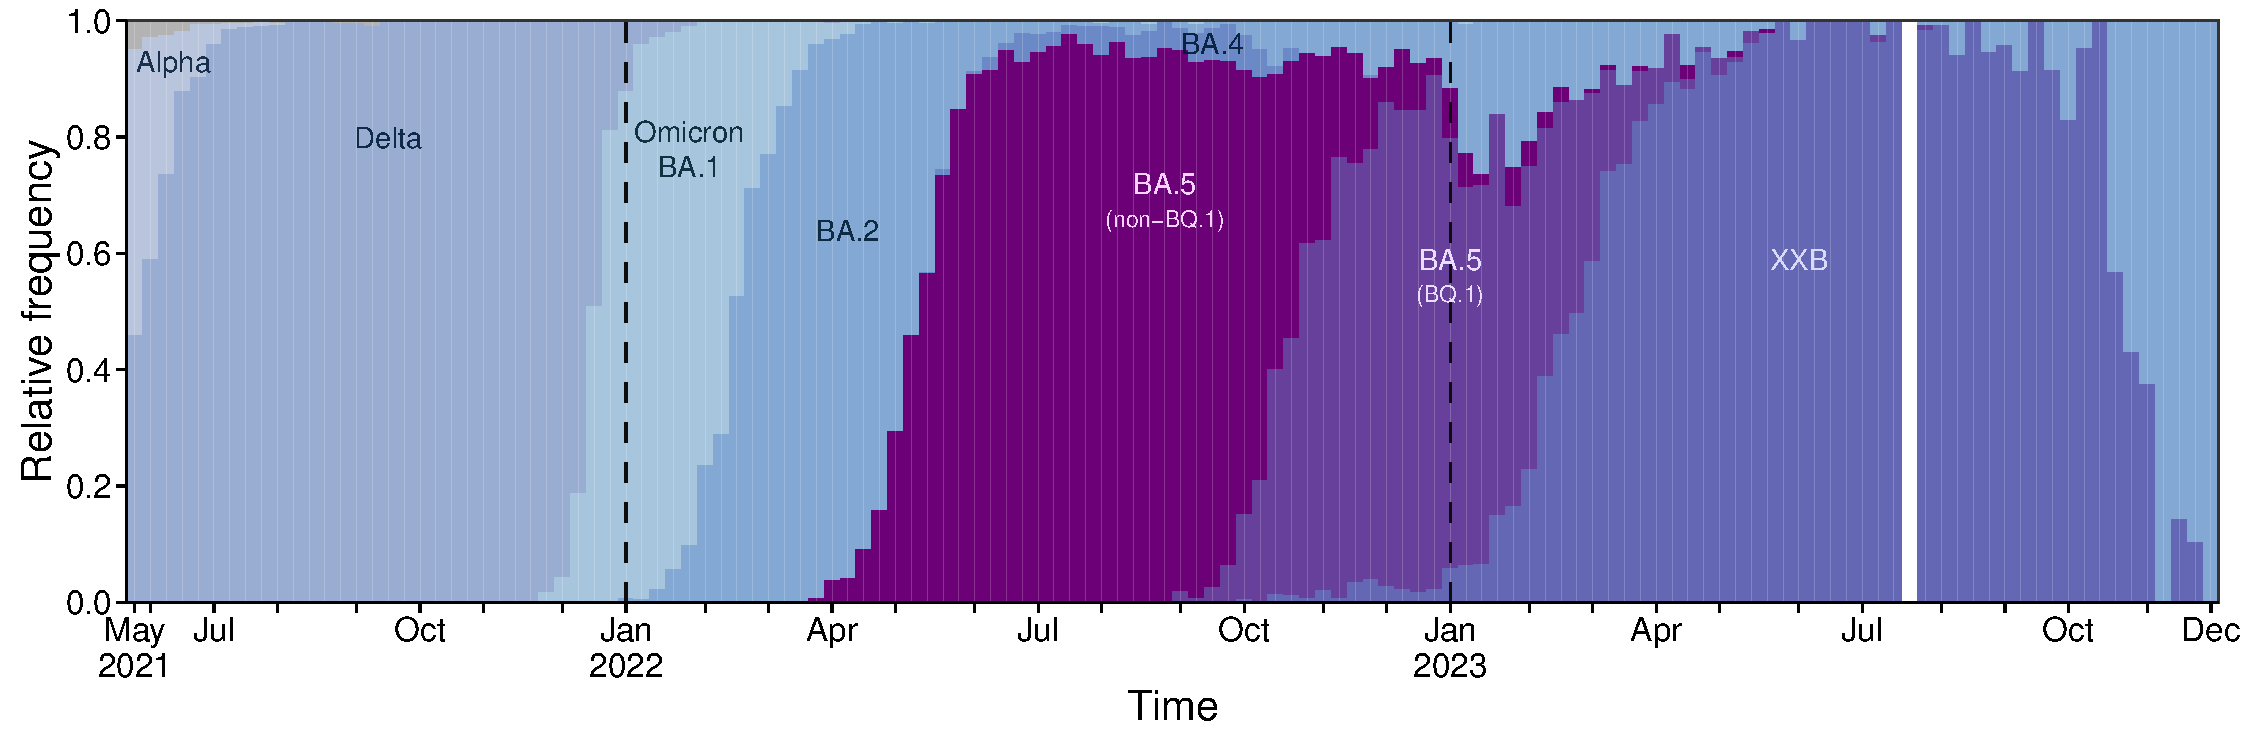
\includegraphics[width=\textwidth]{chapter/introduction/figures/fig1-sarscov2-genetic-diversity-pt.pdf}
    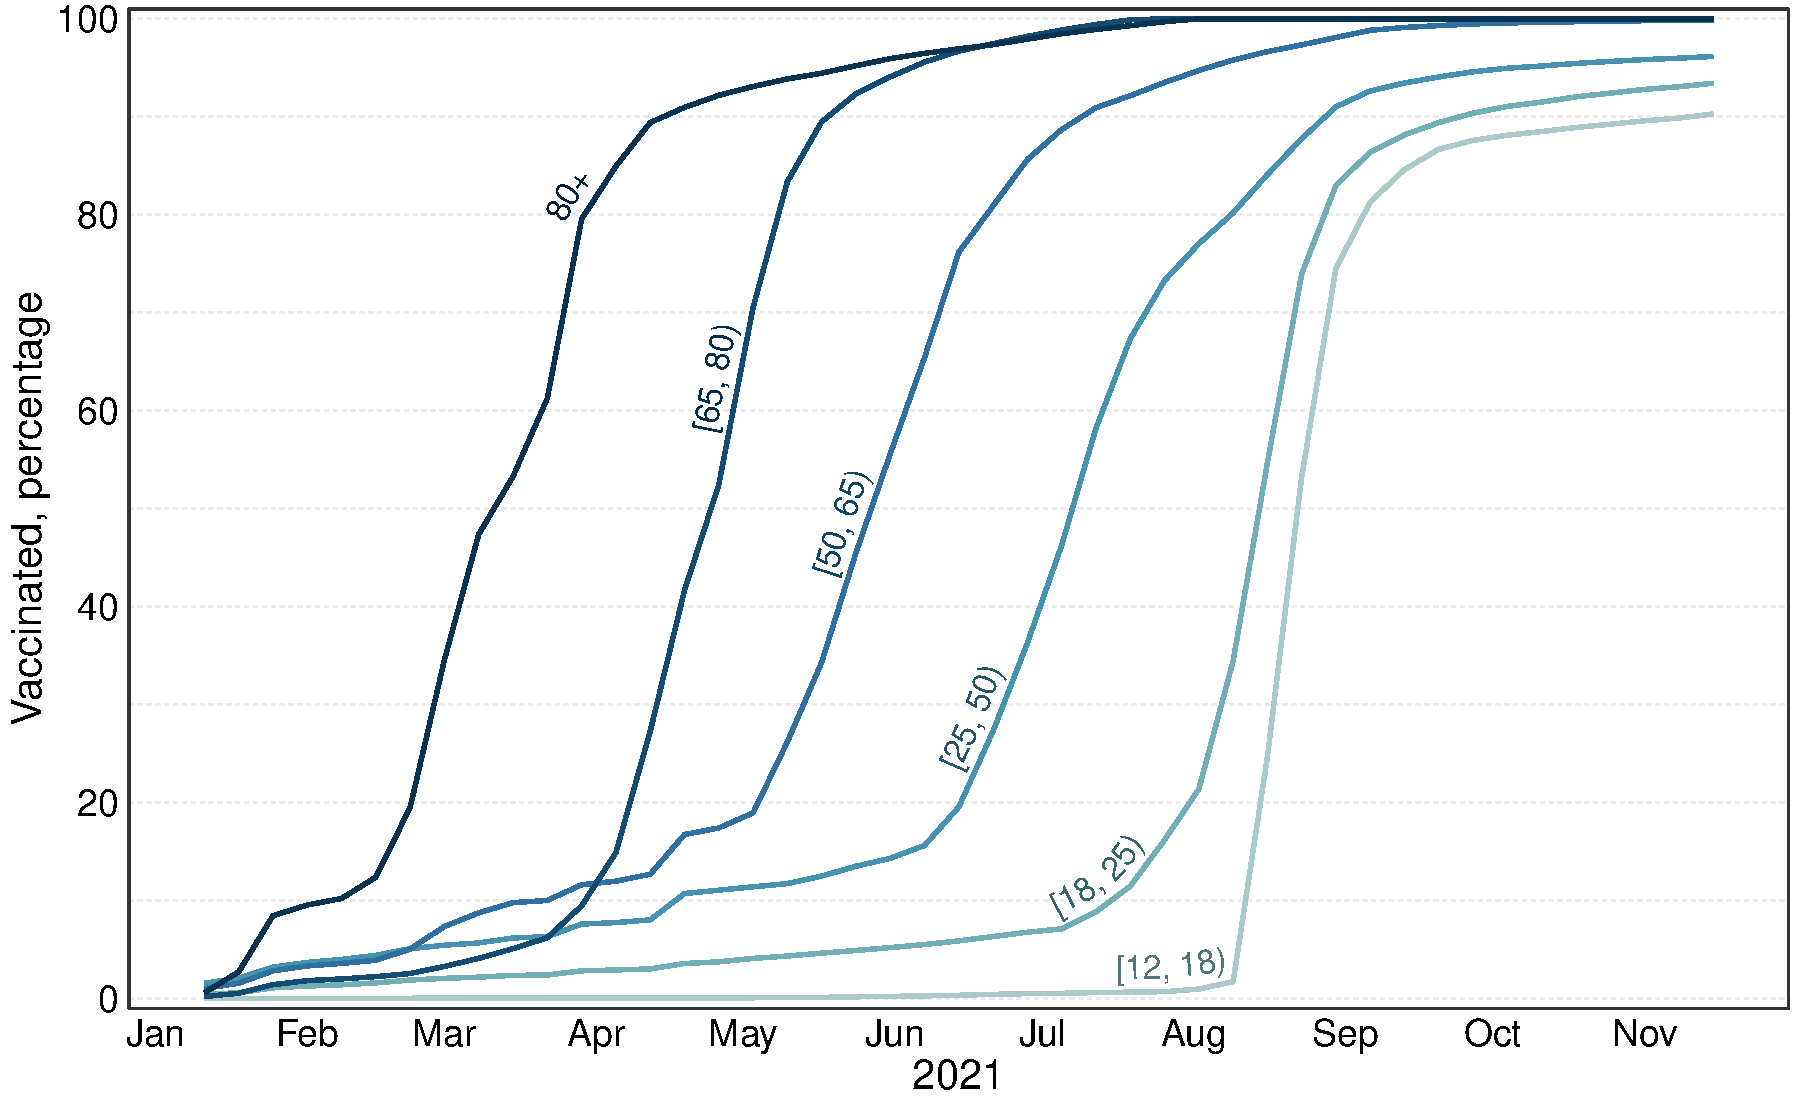
\includegraphics[width=0.8\textwidth]{chapter/introduction/figures/2021-vaccination-percent-agegroup.pdf}
    \caption[Total percentage of vaccine coverage among Portuguese residents by age groups]{Total percentage of vaccine coverage among Portuguese residents by age groups. Available date ranges: Jan 11 2021 to Nov 15 2021. Source: \citet{nationaldirectorateofhealth2021COVID19Vaccination}.}
    \label{fig:intro-vaccination-percentages}
\end{figure}
% Figure 2
% Figure~\ref{fig:intro-vaccination-percentages}

%%%%%%%%%%%%%%%%%%%%%%%%%%%%%%%%%%%%%%%%%%%%%%%%%%%%%%%%%%%%%%%%%%%%%%%%
%%%%%%%%%%%%%%%%%%%%%%%%%%%%%%%%%%%%%%%%%%%%%%%%%%%%%%%%%%%%%%%%%%%%%%%%
\subsection{SARS-CoV-2 variants}

RNA viruses, including \sars, exhibit a considerable rate of genomic mutation, leading to the possible emergence of more adapted variants capable of evading detection and neutralisation by the immune system \citep{markov2023EvolutionSARSCoV2}.
Particularly, the spike protein of these viruses undergoes frequent mutations, allowing for adaptations in the binding affinity towards the human ACE2 receptor \citep{singh2021OriginEvolution}.
% The SARS-CoV-2 has an estimated mutation rate between $1 \times 10^{-6}$ and $2 \times 10^{-6}$ mutations per nucleotide per replication cycle \citep{markov2023EvolutionSARSCoV2}.
With time and multiple recombinations, new sub-variants of \covid with a strong selective advantage became dominant (Figure~\ref{fig:sars-mutations}).
There is a myriad of \sars lineages considered variants of concern (VOC), including Alpha, Delta, and Omicron.
\red{extend the list of variants?}

% 2. mutation rate
% The continues to evolve under 
% The more significant global variants identified were the alpha, beta, gamma, delta and omicron.
% % 3. Omicron and dominant variants
% % 4. assessing risk of infections by new variants in hybrid populations

\begin{figure}[h]
    \centering
    % 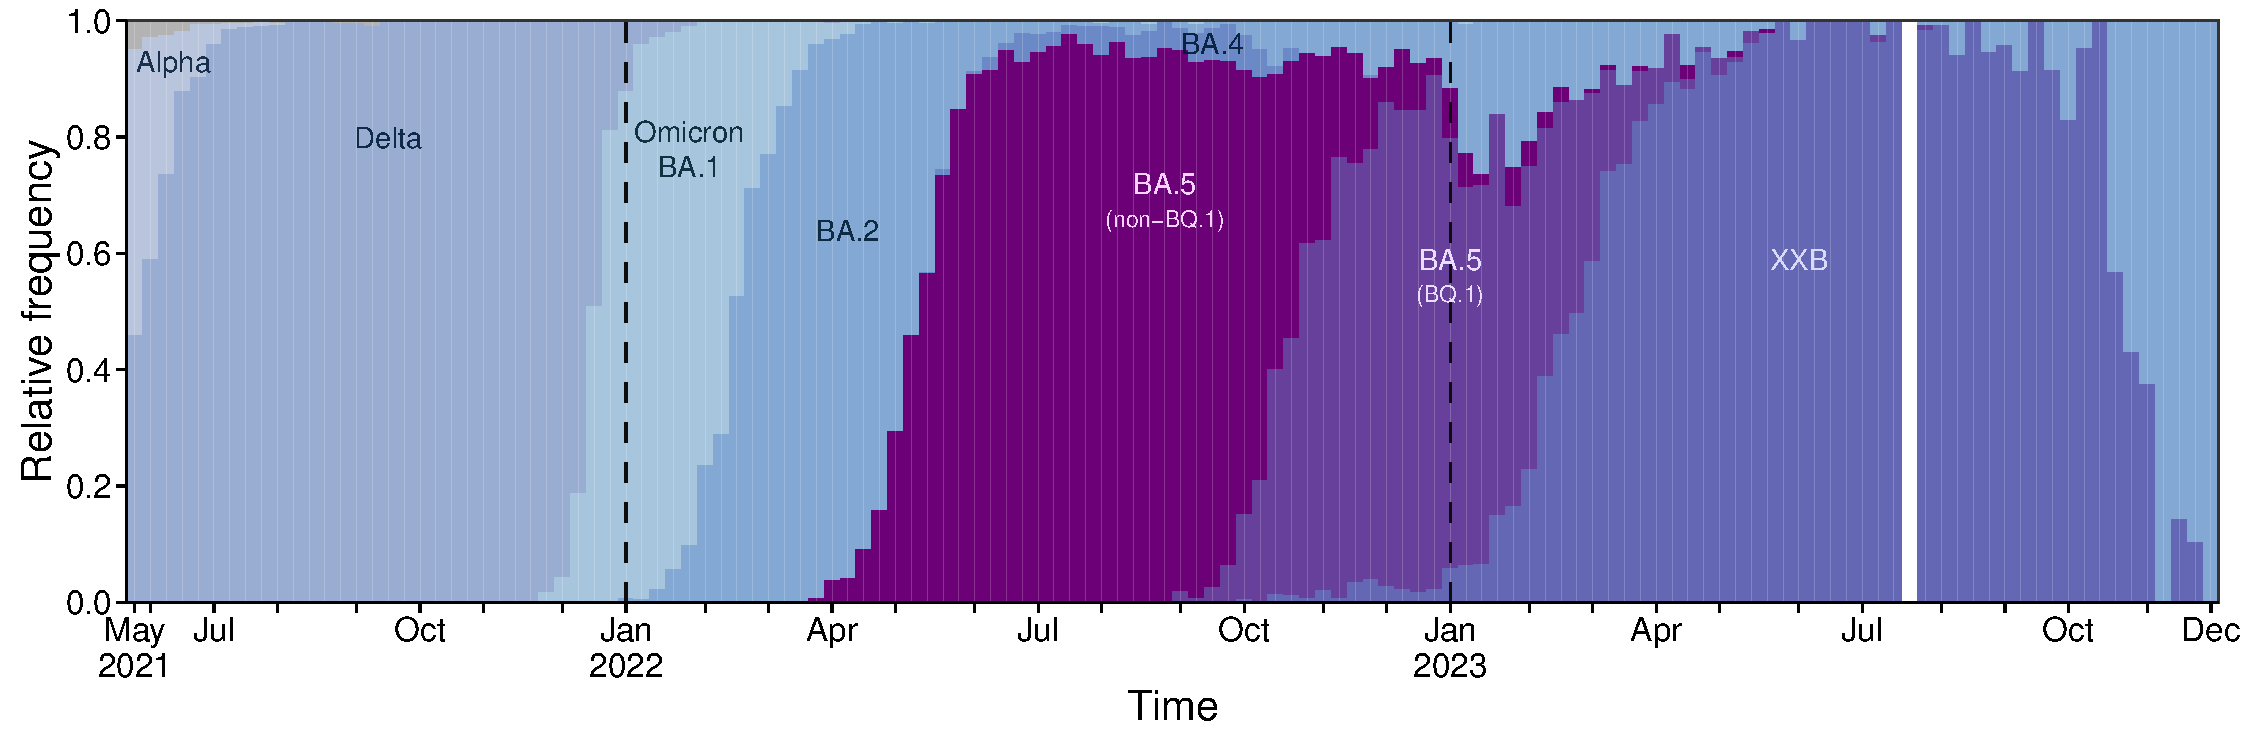
\includegraphics[width=\textwidth]{chapter/introduction/figures/fig1-sarscov2-genetic-diversity-pt.pdf}
    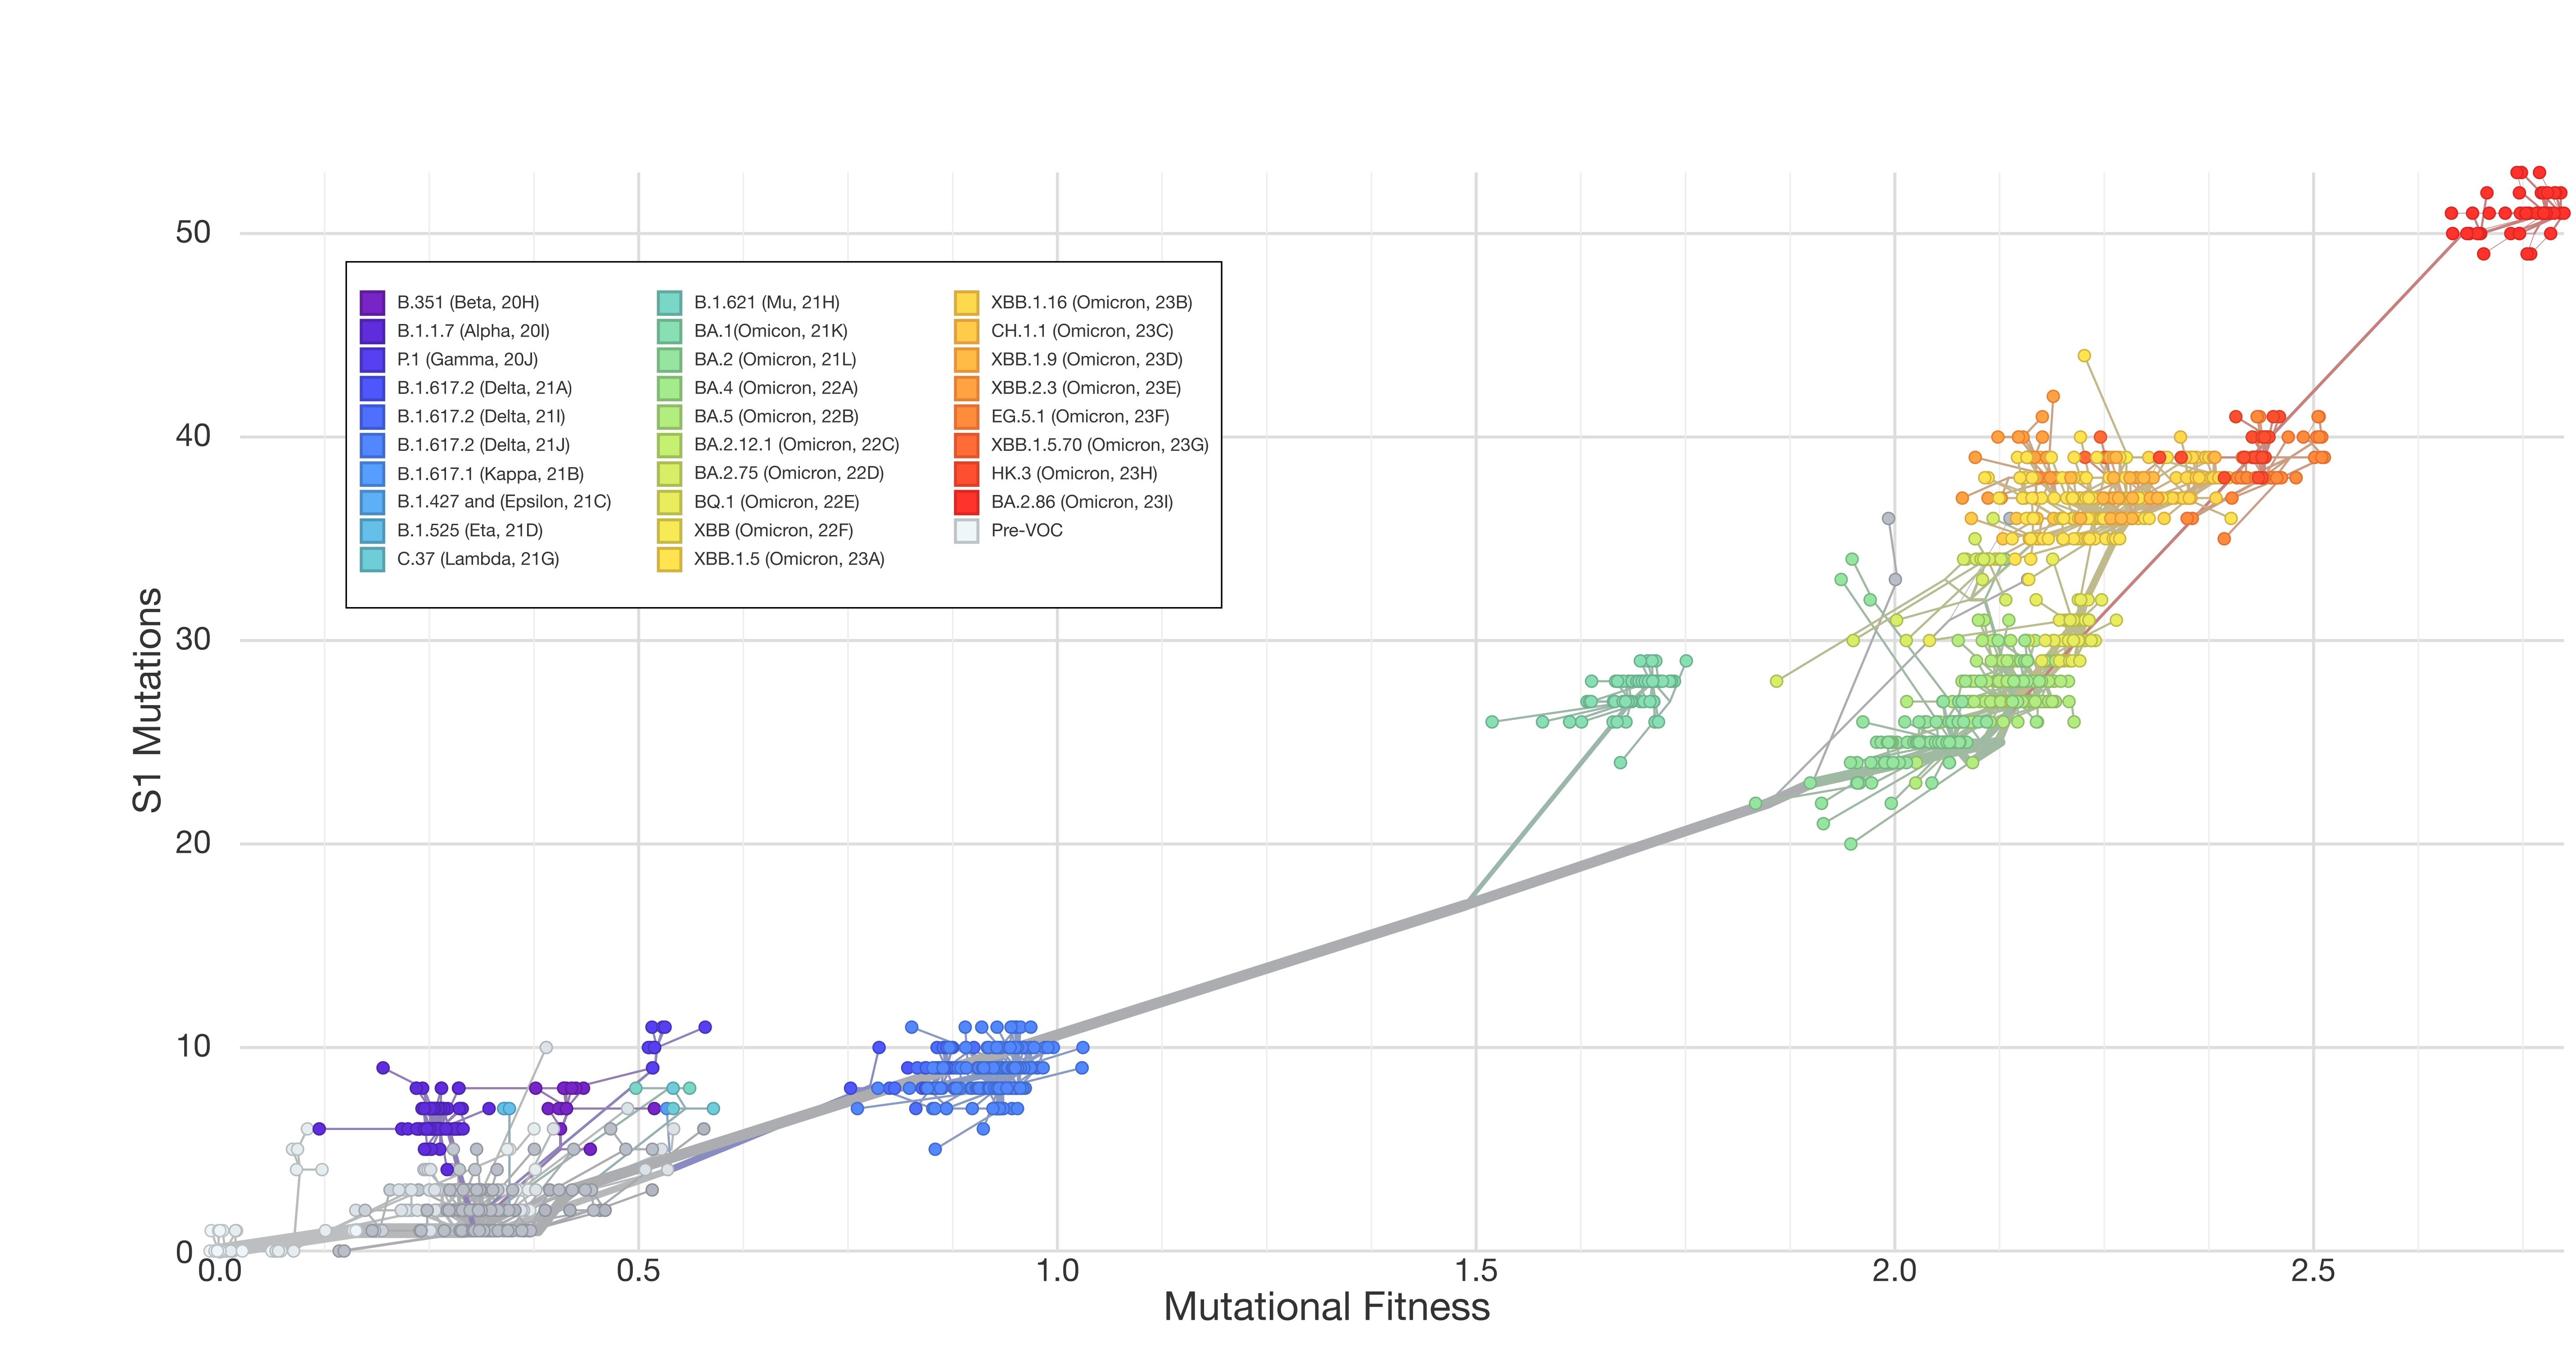
\includegraphics[width=\textwidth]{chapter/introduction/figures/nextstrain_ncov_gisaid_europe_all-time.png}
    \caption[\sars accumulation of amino acid mutations in the spike protein's S1 subunit as a function of their relative mutational fitness]{\sars accumulation of amino acid mutations in the spike protein's S1 subunit as a function of their relative mutational fitness, shown for 2,322 European genomes sampled between December 2019 and December 2023. Generated by \href{https://nextstrain.org/}{nextstrain.org} \citet{hadfield2018NextstrainRealtime}.}
    \label{fig:sars-mutations}
\end{figure}
% Figure 2
% Figure~\ref{fig:sars-mutations}


% ----------------------------------------------------------------------
\subsubsection{Omicron}

% This was the case of the Omicron variant, which was first detected in the Republic of Botswana at the end of 2021 
% reached global dominance 
The Omicron (B.1.1.529) variant was first detected at the end of 2021 in the Republic of Botswana and rapidly raised concerns, due to its much higher capacity to cause reinfections compared to any other preceding variant \citep{pulliam2022IncreasedRisk}.
With multiple mutations in the spike protein, Omicron sub-variants had higher affinity to the ACE2 receptor, its primary cell entry route \citep{starr2020DeepMutational}.
This increased affinity capacitated the sub-variants to more effectively evade antibody binding and neutralisation from naturally- and vaccination-acquired immunity \citep{arora2022AugmentedNeutralisation, greaney2021CompleteMapping}.
And none was more concerning than the sub-variant BA.5 \citep{cao2022BA12}.
\red{Contextualise the state of vaccine development at the time?}


% ----------------------------------------------------------------------
\subsubsection{Omicron in Portugal}

In Portugal, the initial Omicron sub-variants BA.1 and BA.2 quickly became dominant at the start of 2022, first one (BA.1 period of dominance: Jan 1 2022--Feb 6 2022), then the other (BA.2 period of dominance: Mar 27 2022--Apr 17 2022), with a slow transition period between the two \citep{malatoRiskBAInfection2022}.
Between January and February alone, Portugal documented 1.97 million infections, surpassing the total number of cases recorded during the entire epidemic until that period and highlighting the ongoing challenges posed by these variants.

Then, by mid-2022, Portugal became one of the first countries to have Omicron BA.5 as a dominant variant (Figure~\ref{fig:intro-sarscov2-genetic-diversity-pt}).
And despite a majority of the population having received at least one vaccine dose (Figure~\ref{fig:intro-vaccination-percentages}), the sudden rise in cases for this particular lineage was concerning.
% Even if, over 98\% of the Portuguese residents over 12 years old had received at least one vaccine dose at that time (Figure~\ref{fig:intro-vaccination-percentages}), the sudden rise in cases for this particular lineage was concerning.

\begin{figure}[h]
    \centering
    % 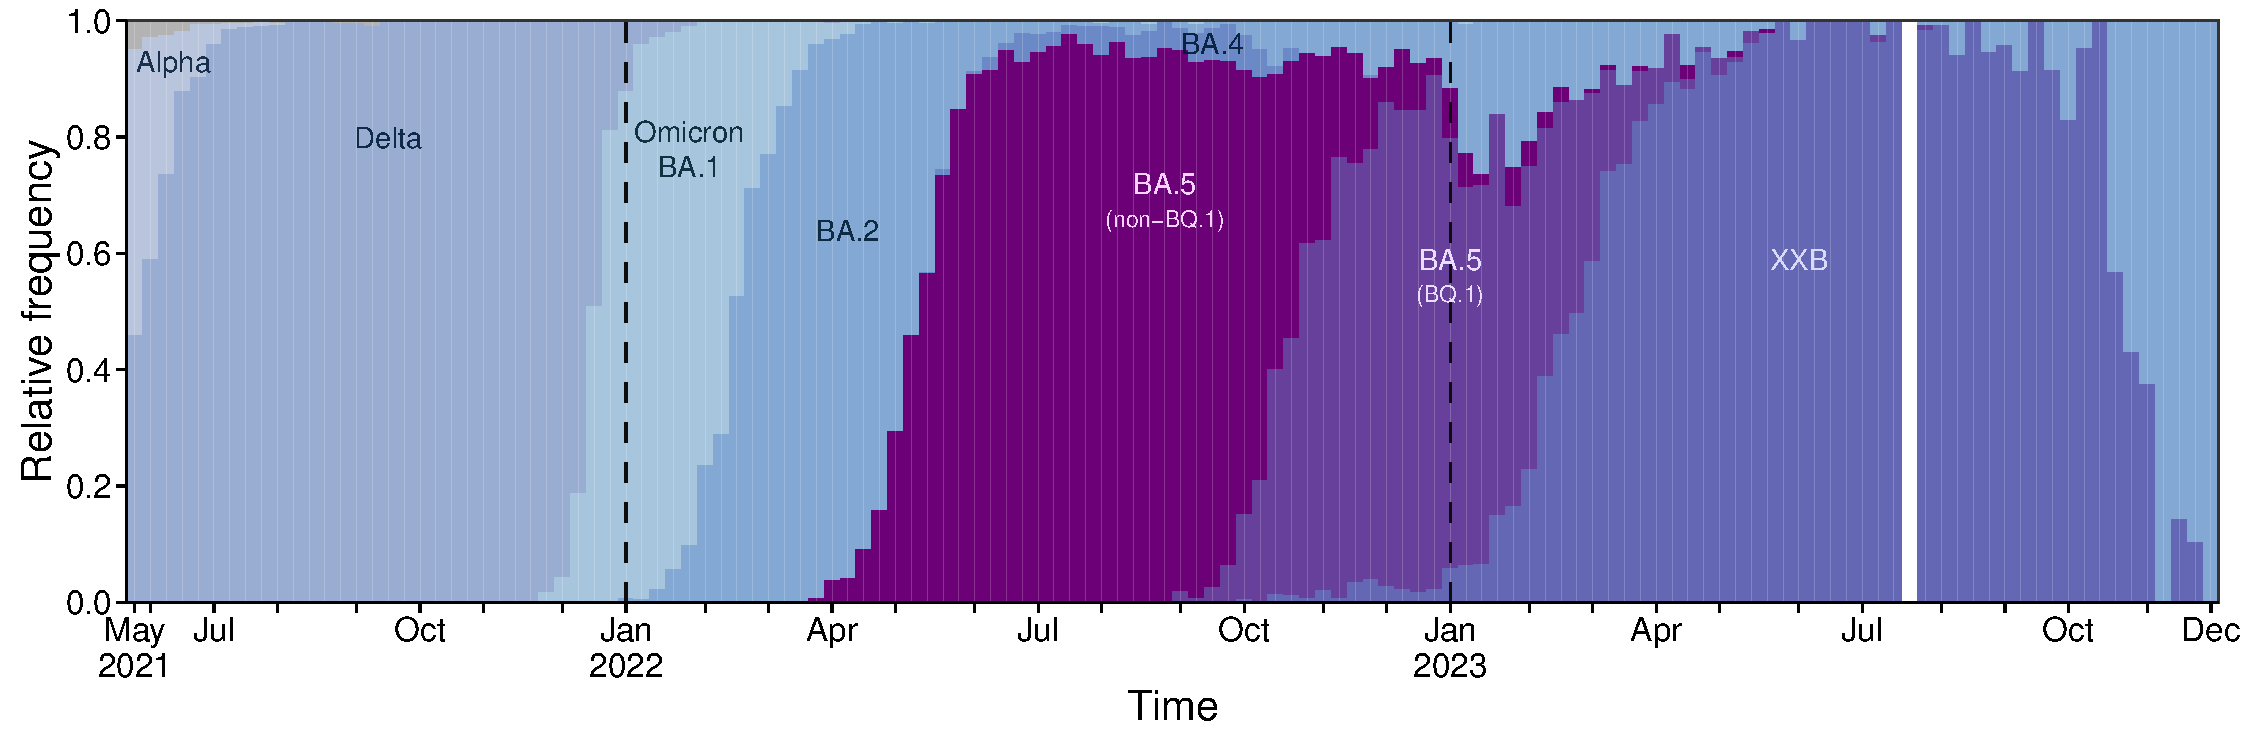
\includegraphics[width=\textwidth]{chapter/introduction/figures/fig1-sarscov2-genetic-diversity-pt.pdf}
    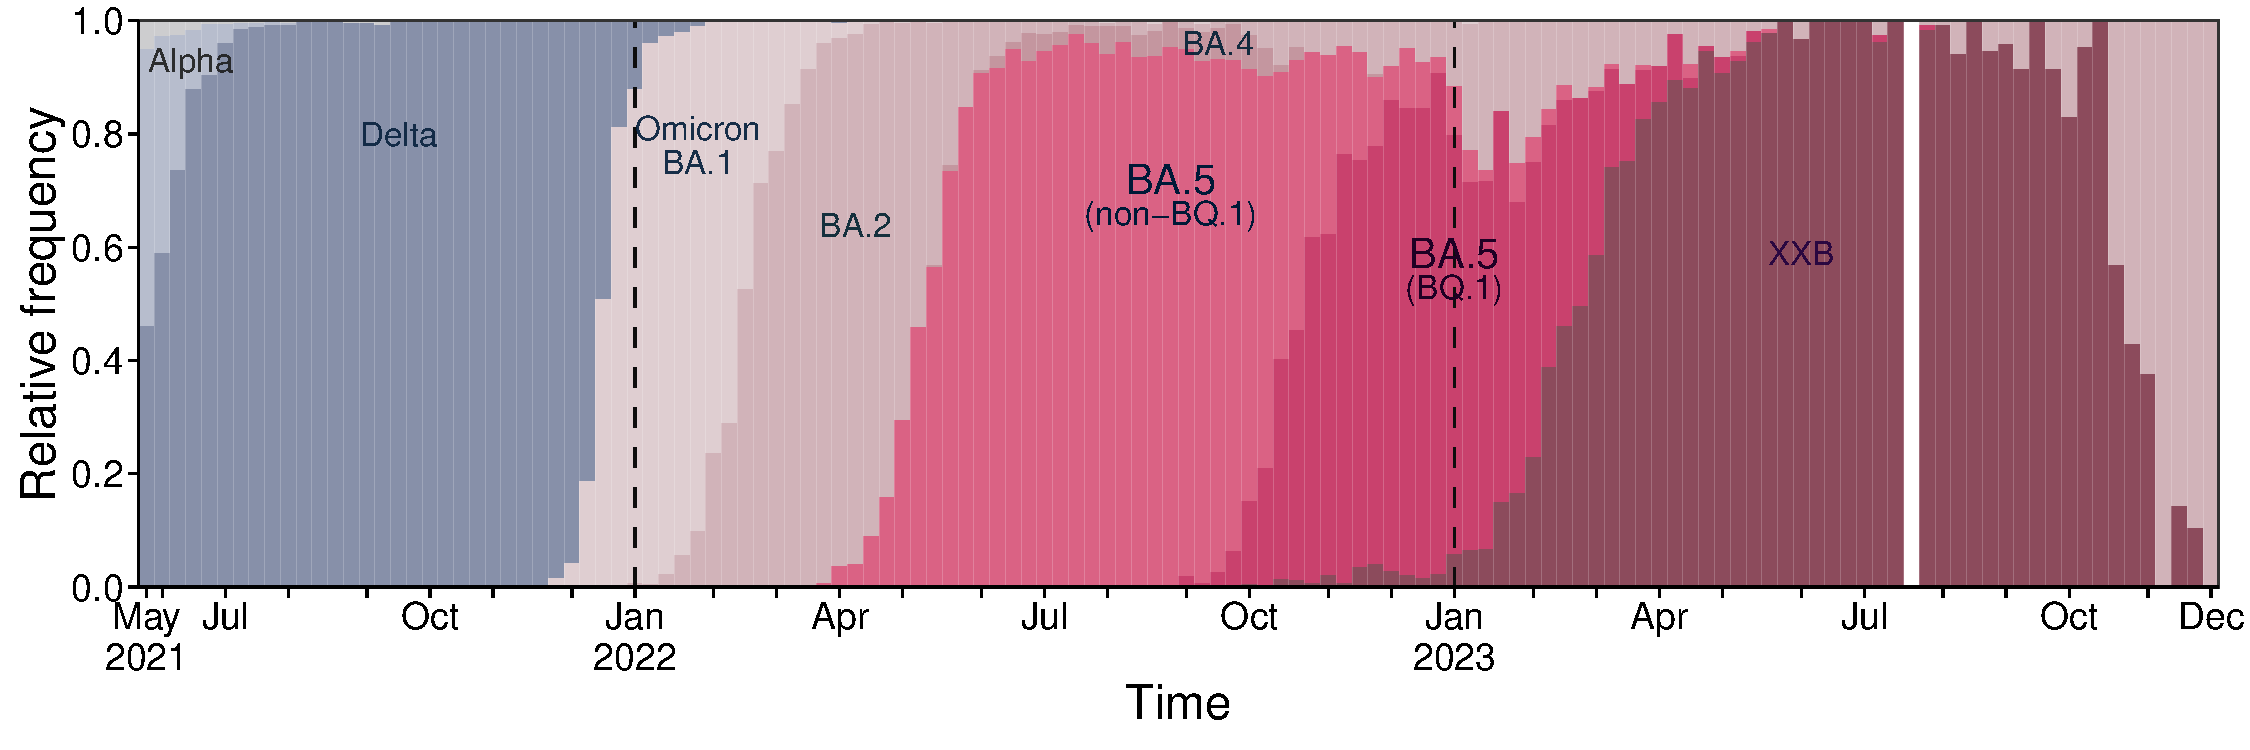
\includegraphics[width=\textwidth]{chapter/introduction/figures/fig1-sarscov2-genetic-diversity-pt03.pdf}
    \caption[Weekly relative frequency of most dominant SARS-CoV-2 variants in Portugal between May 2021 and December 2023]{Weekly relative frequency of the most dominant SARS-CoV-2 variants in Portugal between May of 2021 (week 22) and December of 2023 (week 49). Gray-filled values indicate other variants. Dashed vertical lines indicate the start of 2022 and 2023. Columns left in white represent missing values on particular weeks. Source: \citet{institutonacionaldesaudedoutorricardojorge2023GeneticDiversity}.}
    \label{fig:intro-sarscov2-genetic-diversity-pt}
\end{figure}
% Figure 3
% Figure~\ref{fig:intro-sarscov2-genetic-diversity-pt}

% In Portugal there have been little over 5.6 million cases as of early 2024 (54,765 cases per 100,000 individuals) and 27,906 reported deaths \citep{worldhealthorganization2023WHOCoronavirus}.
% The 

\red{[Finish this]}

% Comparing hybrid and regular \covid vacine-induced immunity \citep{huang2022ComparingHybrid}

% Estudar o risco de infecção/reinfeção em contexto de populações híbridas.

%%%%%%%%%%%%%%%%%%%%%%%%%%%%%%%%%%%%%%%%%%%%%%%%%%%%%%%%%%%%%%%%%%%%%%%%
%%%%%%%%%%%%%%%%%%%%%%%%%%%%%%%%%%%%%%%%%%%%%%%%%%%%%%%%%%%%%%%%%%%%%%%%
%%%%%%%%%%%%%%%%%%%%%%%%%%%%%%%%%%%%%%%%%%%%%%%%%%%%%%%%%%%%%%%%%%%%%%%%
\section{Aims of the thesis}
\label{sec:aims-thesis}
% Obrigatório ter esta secção na these.
% Thesis: estratificação em grupos mais homogénios e mecanisticamente similares a fim de poder desenvolver metodologias de tratamento personalizadas.

% \textbf{Part~\ref{part:introduction}}
% \textbf{Part~\ref{part:mecfs}}
% \textbf{Part~\ref{part:covid}}
% \textbf{Part~\ref{part:discussion}}

% \textbf{Chapter~\ref{chapter:introduction}}
% \textbf{Chapter~\ref{chapter:statical-challenges-2021}}
% \textbf{Chapter~\ref{chapter:misdiagnosis-serology-2022}}
% \textbf{Chapter~\ref{chapter:impact-misdignosis-2023}}
% \textbf{Chapter~\ref{chapter:}}
% \textbf{Chapter~\ref{chapter:2022-revisiting-igg}}
% \textbf{Chapter~\ref{chapter:2023-sym-and-herpesvirus}}
% \textbf{Chapter~\ref{chapter:2021-ace-ace2}}
% \textbf{Chapter~\ref{chapter:2022-covid19-01}}
% \textbf{Chapter~\ref{chapter:2023-covid19-02}}
% \textbf{Chapter \ref{chapter:discussion}}

The work presented in this thesis is related to both topics of \cfs and \covid.
Apart from the single-chapter parts concerning the general introduction (\textbf{Part~\ref{part:introduction}} with \textbf{Chapter~\ref{chapter:introduction}}) and general discussion (\textbf{Part~\ref{part:discussion}} with \textbf{Chapter \ref{chapter:discussion}}), the thesis is divided into two parts.

The overarching themes discussed in \textbf{Part~\ref{part:mecfs}} encompass reproducibility in \cfs research and the stratification of diagnosed patients into more homogeneous and mechanistically similar subgroups. This approach aims to help identify potential weaknesses in biomarker research related to patient misdiagnosis and improve the consistency of study results, gradually increasing the understanding of the disease. At the same time, this work demonstrates the importance of sound statistical methodologies.

\begin{enumerate}
    \setlength{\itemsep}{1.5pt}
    \setlength{\parskip}{0pt}
    \setlength{\parsep}{0pt}
    
    % \textbf{Chapter~\ref{chapter:statical-challenges-2021}}
    \item Diagnosis of \cfs is done through symptom-base criteria with multiple different case definitions that can diagnose different individuals as suspected cases. Additionally, an overlap of symptoms and severity has been described between \cfs-diagnosed individuals and other fatigue-inducing diseases. Work done in \textbf{Chapter~\ref{chapter:statical-challenges-2021}} uses data from the specialised UK ME/CFS Biobank (UKMEB) to study the lack of diagnostic agreement between four of the most commonly used \cfs case definitions and the similarity of symptoms among patients and different control groups. The study also presents the initial ideas on the impact of misdiagnosis (or misclassification) on patients.

    % \textbf{Chapter~\ref{chapter:misdiagnosis-serology-2022}}
    % \textbf{Chapter~\ref{chapter:impact-misdignosis-2023}}
    \item \textbf{Chapter~\ref{chapter:misdiagnosis-serology-2022}} and \textbf{Chapter~\ref{chapter:impact-misdignosis-2023}} extend the previous ideas of disease uncertainty and patient heterogeneity and simulate scenarios of case-control studies assuming possible inclusion of false positives (i.e., misdiagnosed) patients to estimate the reduction in statistical the power to detect an association to a candidate causal factor. The former is a hypothetical application, extrapolating on the link between \cfs and viral infections to use data from three \covid seroepidemiological studies. The latter describes the idea of misdiagnosis with more detail, performing simulations under different parametric conditions. Moreover, it analyses available data on candidate genetic and serological markers for \cfs and studies the reproducibility of the published results under the proposed assumption of inherent patient misdiagnosis.

    % \textbf{Chapter~\ref{chapter:}}
    \item \red{Added chapter: Proposed work on the stratification of ME/CFS individuals through the creation of specific symptomatological profiles related to seven different domains and possible pathologies.}

    % \textbf{Chapter~\ref{chapter:2022-revisiting-igg}}
    \item There is a growing body of evidence linking EBV infection as a trigger to the pathogenesis of a subgroup of \cfs individuals, with possible antigen mimicry as the root of an autoimmune response. \textbf{Chapter~\ref{chapter:2022-revisiting-igg}} re-analyses antibody-wide association analysis data from a previous study on IgG antibody responses against antigens derived from 14 EBV proteins \citep{loebel2017SerologicalProfiling}. Different regression models are built, relating antibody levels with both age and gender, with \cfs patients stratified into infection trigger-specific subgroups and compared with matched healthy controls.
    % The study founds two candidate antigens inducing increased antibody responses in ME/CFS patients with an infectious trigger that could be used for diagnosis of this particular subgroup

    % \textbf{Chapter~\ref{chapter:2023-sym-and-herpesvirus}}
    \item \cfs and MS patients share a large number of symptoms and the onset of both diseases is linked with an acute viral infection. To better understand the differences between \cfs and MS, their reported symptoms, and their relation to viral agents, \textbf{Chapter~\ref{chapter:2023-sym-and-herpesvirus}} re-analyses data from the UKMEB to report the underlying association between the profile of symptoms and concentration of IgG antibody responses to six herpesviruses (CMV, EBV, HHV6, HSV1, HSV2, and VZV) on a population of MS controls and ME/CFS. Following the previous studies in this thesis, ME/CFS patients are stratified based on reported infection triggers. Furthermore, the study also tries to discriminate between the ME/CFS subgroups and MS, using different models and link functions.

    % \textbf{Chapter~\ref{chapter:2021-ace-ace2}}
    \item The \sars entry into the human cells is mediated by the ACE2 receptors and complications associated with the disease have been linked with the down-regulation of this enzyme. Thus, individuals with a baseline ACE2 deficiency are potentially at an increased risk of developing \covid and harsh inflammatory responses. To assess whether \cfs patients have increased susceptibility to \covid, \textbf{Chapter~\ref{chapter:2021-ace-ace2}} performs a meta-analysis of public CpG DNA methylation and gene expression data for ACE2 and its homologous ACE protein.
\end{enumerate}

\textbf{Part~\ref{part:covid}} was done throughout the second half of 2022, in the context of the \covid pandemic and the rise of progressively more dominant \sars Omicron sub-variants in highly vaccinated populations.
% The two chapters here included were developed in parallel with the remaining project of the thesis.
% The combined output from the two studies was distinguished with the 2023 ``Pfizer Award for Clinical Research''.

\begin{enumerate}
    \setlength{\itemsep}{1.5pt}
    \setlength{\parskip}{0pt}
    \setlength{\parsep}{0pt}
    \setcounter{enumi}{6}

    % \textbf{Chapter~\ref{chapter:2022-covid19-01}}
    \item By mid-2022 it became important to understand the impact of previous infections on the risk of infection and reinfection posed by the Omicron BA.5 sub-variant. \textbf{Chapter~\ref{chapter:2022-covid19-01}} makes use of the Portuguese \covid registry and the national \sars genetic surveillance data to identify the periods of dominance for previous VOC and Omicron sub-variants (BA.1 and BA.2) and assesses how infections during those periods (representing adapted vaccines to these dominant variants) can be effective against BA.5.
    % \textbf{Chapter~\ref{chapter:2022-covid19-01}} \citep{malatoRiskBAInfection2022} compares the Omicron BA.5 sub-variant infection risk in vaccinated and hybrid (vaccinated + prior single infection with other VOC) individuals to demonstrate how vaccines adapted to other sub-variants of Omicron can effectively reduce the risk of reinfection.

    % \textbf{Chapter~\ref{chapter:2023-covid19-02}}
    \item Following the results of the previous chapter, \textbf{Chapter~\ref{chapter:2023-covid19-02}} uses the same data to study how the hybrid immunity (vaccine + single BA.1/BA.2 infection) effectiveness of protection against a BA.5 infection decays over time.
\end{enumerate}


%%%%%%%%%%%%%%%%%%%%%%%%%%%%%%%%%%%%%%%%%%%%%%%%%%%%%%%%%%%%%%%%%%%%%%%%
% \subsubsection{Contextualisation to the reader}
% \textbf{Part~\ref{part:introduction}}
% \textbf{Part~\ref{part:mecfs}}
% \textbf{Part~\ref{part:covid}}
% \textbf{Part~\ref{part:discussion}}

% \textbf{Chapter~\ref{chapter:introduction}}
% \textbf{Chapter~\ref{chapter:statical-challenges-2021}}
% \textbf{Chapter~\ref{chapter:misdiagnosis-serology-2022}}
% \textbf{Chapter~\ref{chapter:impact-misdignosis-2023}}
% \textbf{Chapter~\ref{chapter:}}
% \textbf{Chapter~\ref{chapter:2022-revisiting-igg}}
% \textbf{Chapter~\ref{chapter:2023-sym-and-herpesvirus}}
% \textbf{Chapter~\ref{chapter:2021-ace-ace2}}
% \textbf{Chapter~\ref{chapter:2022-covid19-01}}
% \textbf{Chapter~\ref{chapter:2023-covid19-02}}
% \textbf{Chapter \ref{chapter:discussion}}

Most chapters presented in this thesis correspond to already published peer-reviewed scientific articles, and the document is ordered as to make it clearer for the reader rather than the chronological order of publication.

In \textbf{Part~\ref{part:mecfs}}, both studies from \textbf{Chapter~\ref{chapter:statical-challenges-2021}} \citep{malato2021Statisticalchallenges} and \textbf{Chapter~\ref{chapter:misdiagnosis-serology-2022}} \citep{malato2022ImpactMisclassification} were originally prepared for publication in the Proceedings of the Portuguese Statistical Society, which also employs a peer-review system.
The first study provides an introduction to the overall challenges related to agreement in \cfs diagnosis and patient heterogeneity, briefly mentioning the possible impact of misdiagnosis (described as ``misclassification'').
In fact, the ideas on the impact of misdiagnosis began to take shape during the preparation of this work.
The second study serves as a hypothetical exercise to the notions of patient and serological tests' misdiagnosis.
Ultimately, the concepts proposed in both articles were further developed and formalised, eventually being published in the article presented in \textbf{Chapter~\ref{chapter:impact-misdignosis-2023}} \citep{malato2023ImpactMisdiagnosis}.
This comes as a brief note that while some of the proposed mathematical assumptions might differ from one chapter to the next, the equations discussed remain the same overall.

The two chapters included in \textbf{Part~\ref{part:covid}} (\textbf{Chapter~\ref{chapter:2022-covid19-01}} and \textbf{Chapter~\ref{chapter:2023-covid19-02}}) were developed in parallel with the remaining project of the thesis.
The resulting papers are correspondence articles that give an insight into the period of uncertainty regarding whether or not vaccines adapted to past lineages---particularly Omicron BA.1, which was under development at the time---would provide effective and enduring protection towards the new dominant Omicron BA.5 sub-variant \citep{malatoRiskBAInfection2022, malato2023StabilityHybrida}.

Minor editorial adjustments were made to clarify the chapters and homogenise the overall consistency of this thesis.
% As required by the Faculty's presentation rules, t
The original published articles are included \textit{facsimile} in the Appendices (\textbf{Part \ref{appendix:appendix}}).

To conclude, \textbf{Chapter~\ref{chapter:discussion}} (\textbf{Part~\ref{part:discussion}}) provides a general discussion of the most important aspects of this thesis, with highlights on the main achievements and final remarks and potential future work. \red{[provide clear examples on the discussed topics?]}
% Namely, how the consideration of patient misdiagnosis could represented


% \vfill
% \newpage
%%%%%%%%%%%%%%%%%%%%%%%%%%%%%%%%%%%%%%%%%%%%%%%%%%%%%%%%%%%%%%%%%%%%%%%%
\addcontentsline{toc}{section}{Bibliography}
\bibliographystyle{abbrvnat}
\bibliography{references}
%%%%%%%%%%%%%%%%%%%%%%%%%%%%%%%%%%%%%%%%%%%%%%%%%%%%%%%%%%%%%%%%%%%%%%%%